\documentclass[twoside, doctor]{HTU-thesis-grd}
%模板选项： 硕士论文 master； 博士论文 doctor
%oneside选项表示单页打印,twoside选项表示双页打印. 默认单面打印 oneside,硕士论文模板 master
%==============更改数学字体设置，Latin Modern Math 默认的的确有点细，看个人需要，下面提供一种方法，需要的可以取消注释=========%
% \usepackage[bold-style=ISO]{unicode-math} %采用unicode-math，可以直接输入Unicode公式，当然传统的输入就行
% \setmathfont{XITS Math}  %目前unicode-math 支持几种数学字体，具体用法可以查看帮助文档，这里采用类似times字体科学数学字体，可以取消注释对比
\usepackage{amsmath,amsfonts}
\usepackage{algorithm, algorithmicx, algpseudocode}
\usepackage{amssymb}
\usepackage{subcaption}
\begin{document}

% 中文封面内容

% 单位代码
\institutenumber{10476}
 
% 学号
\confidential{2308283080}

% 分类号
\classification{TP18}

% 中文题目
\title{硬件损伤条件下去蜂窝大规模 MIMO 系统性能研究}

% 专业学位领域
\major{计算机技术}

% 专业学位类别
\degree{工学硕士}

% 申请人
\author{李世龙}

% 指导教师
\advisor{周猛 ~~ 教授}



\interest{***}


\defenddate{二〇二六年五月}

% 英文封面内容
\englishtitle{Performance analysis of cell free massive MIMO system based on reinforcement learning under hardware impairment}
\englishauthor{\emph{Shilong Li}}
\englishadvisor{Prof. Meng Zhou}
\englishdate{May, 2026}

% 首页封面绘制
%\maketitle

% 中文标题页绘制
\makeInfo

% 英文标题页绘制
\makeEnglishInfo



%%%%%%%%%%%%前置部分%%%%%%%%%%%%
\frontmatter

% 摘要
\begin{abstract}
去蜂窝大规模多输入多输出（CF-mMIMO）系统通过密集部署大量接入点（AP），可实现无缝通信覆盖，显著提升用户频谱效率与系统总容量。然而，该架构在实际部署中面临高昂的成本压力，且不可避免地引入非理想硬件因素。本文针对上述挑战，系统研究了非理想硬件条件下CF-mMIMO系统的资源分配与性能优化问题。

具体而言，本文首先研究了在用户设备（UE）端模拟非线性功率放大器（PA）及AP端采用低分辨率模数转换器（ADC）条件下，上行CF-mMIMO系统的可达速率性能。推导了上行用户可达速率的闭式表达式，系统分析了AP数量、UE密度、AP天线数目及ADC分辨率等关键参数对系统性能的影响。为有效抑制UE间干扰并提升系统和速率，提出了一种基于图神经网络（GNN）辅助的演员-评论家（Actor-Critic）功率分配算法（DMAGNN-AC）。该框架突破了深度强化学习在高维非结构化状态空间下的表征瓶颈，实现了具备物理可解释性的特征嵌入。与全功率发射方案相比，所提功率分配策略可使系统速率提升近一倍。进一步地，为缓解低分辨率ADC对系统速率的不利影响，设计了多智能体深度Q集成网络（MADQIN）以优化ADC分辨率分配策略。

在此基础上，本文进一步研究了非理想硬件条件下CF-mMIMO系统的超可靠低时延通信（URLLC）服务资源分配策略。针对工业自动化等物联网关键应用对毫秒级时延与极高可靠性的严苛需求，构建了非线性PA的损伤模型，推导了有限块长下上行链路UE速率闭合表达式。为降低传统优化算法的计算复杂度，提出基于GNN与深度强化学习融合的智能功率控制策略，通过图嵌入技术建模UE空间相关性，动态抑制硬件损伤与时变信道干扰。所提方案在保持毫秒级时延的同时，为工业自动化等物联网应用提供理论与技术支撑。仿真结果充分验证了所提方案的有效性。

\keywords{去蜂窝大规模MIMO; 非理想硬件; 图神经网络; 深度强化学习; 功率分配; 超可靠低时延通信; 有限块长; 资源分配}
%({\color{blue}{一般选3 \textasciitilde 8个单词或专业术语，且中英文关键词必须对应。}})
\end{abstract}

\begin{englishabstract}
Cell-free massive multiple-input multiple-output (CF-mMIMO) systems, characterized by dense deployment of access points (APs), provide seamless communication coverage with significant enhancements in spectral efficiency and overall system capacity. However, the practical implementation of this architecture faces substantial cost challenges and inevitably introduces non-ideal hardware impairments. This dissertation systematically addresses resource allocation and performance optimization challenges in CF-mMIMO systems operating under non-ideal hardware conditions.

This research first investigates the achievable rate performance of uplink CF-mMIMO systems incorporating nonlinear power amplifiers (PAs) at user equipment (UE) terminals and low-resolution analog-to-digital converters (ADCs) at APs. Closed-form expressions for uplink user achievable rates are derived, enabling comprehensive analysis of key system parameters including AP deployment density, UE distribution characteristics, antenna array configurations, and ADC quantization precision. To effectively mitigate inter-user interference and enhance system throughput, a graph neural network (GNN)-assisted actor-critic power allocation algorithm (DMAGNN-AC) is proposed. This framework overcomes the representation limitations inherent in deep reinforcement learning (DRL) when dealing with high-dimensional unstructured channel state information, achieving physically interpretable feature learning. Compared with conventional full-power transmission strategies, the proposed power allocation approach achieves approximately twofold improvement in system rate performance. Furthermore, to alleviate the performance degradation caused by low-resolution ADCs, a multi-agent deep Q-integration network (MADQIN) is designed for optimizing ADC resolution allocation strategies.

Building upon these contributions, this research extends to resource allocation strategies for ultra-reliable low-latency communication (URLLC) services in CF-mMIMO systems with hardware impairments. Addressing the stringent requirements of millisecond-level latency and ultra-high reliability in critical IoT applications such as industrial automation, impairment models for nonlinear PAs are established, and closed-form rate expressions for uplink UEs under finite blocklength constraints are derived. To reduce the computational complexity of traditional optimization algorithms, an intelligent power control strategy integrating GNN with DRL is developed. By leveraging graph embedding techniques to model spatial correlations among UEs, the proposed approach enables dynamic suppression of hardware-induced distortions and time-varying channel interference. The developed solution maintains millisecond-level latency while providing theoretical and technical support for IoT applications in industrial automation. Simulation results comprehensively validate the effectiveness of the proposed methodologies.

\englishkeywords{CF-mMIMO, non-ideal hardware, graph neural network, deep reinforcement learning, power allocation, ultra-reliable low-latency communication, finite blocklength, resource allocation}

\end{englishabstract}


% 加入目录
\tableofcontents

%加入图、表索引(同时取消图表索引中章之间的垂直间隔)
\let\origaddvspace\addvspace
\renewcommand{\addvspace}[1]{}
\listoffigures
\addcontentsline{toc}{chapter}{\heiti{插图索引}}
\listoftables
\addcontentsline{toc}{chapter}{\heiti{表格索引}}
\renewcommand{\addvspace}[1]{\origaddvspace{#1}}

%\RequirePackage[numbers,square,comma,super,sort&compress]{natbib}
% “上标”引用
%\newcommand{\upcite}[1]{\textsuperscript{\cite{#1}}}}


% 参考文献的"文本"引用     “\mycite”
\newcommand{\textcite}[1]{\scalebox{1.3}[1.3]{\raisebox{-0.65ex}{\cite{#1}}}}

% 主要符号对照表
\begin{denotation}

\item [${x}$] 标量${x}$
\item [${{\bf{x}}}$] 列矢量${{\bf{x}}}$
\item [${{\bf{X}}}$] 矩阵${{\bf{X}}}$
\item [${{\bf{X}}}_{m,n}$] 矩阵${\bf{X}}$的第$m$行第$n$列元素
\item [${{\bf{x}}}^*$] 共轭${{\bf{x}}}^*$
\item [${{\bf{x}}}^T$] 转置${{\bf{x}}}^T$
\item [${{\bf{x}}}^H$] 共轭转置${{\bf{x}}}^H$
\item [$\text{diag}({{\bf{A}}})$] 对角矩阵$\text{diag}({{\bf{A}}})$
\item [$|\cdot|$] 绝对值$|\cdot|$
\item [$\|\cdot\|$] 欧几里得范数$\|\cdot\|$
\item [$\mathbb{E}\{\cdot\}$] 期望$\mathbb{E}\{\cdot\}$
\item [$\text{Var}\{\cdot\}$] 方差$\text{Var}\{\cdot\}$
\item [$\text{vec}(\cdot)$] 矩阵向量化$\text{vec}(\cdot)$
\item [${{\bf{I}}}_N$] $N\times N$单位矩阵${{\bf{I}}}_N$
\item [$\sim$] 服从分布$\sim$
\item [$\mathcal{CN}$] 复高斯分布$\mathcal{CN}$

\end{denotation}

% 缩略词列表
\begin{abbreviation}
\item[***] ******, ******
\item[***] ******, ******
\item[***] ******, ******

















\end{abbreviation}


%%%%%%%%%%%%正文主体部分%%%%%%%%%%%%
\mainmatter

%% 各章正文内容

\chapter{绪论}\label{chap:intro}
\section{研究背景和意义}
**********************

\begin{figure}[h]
	\centering
	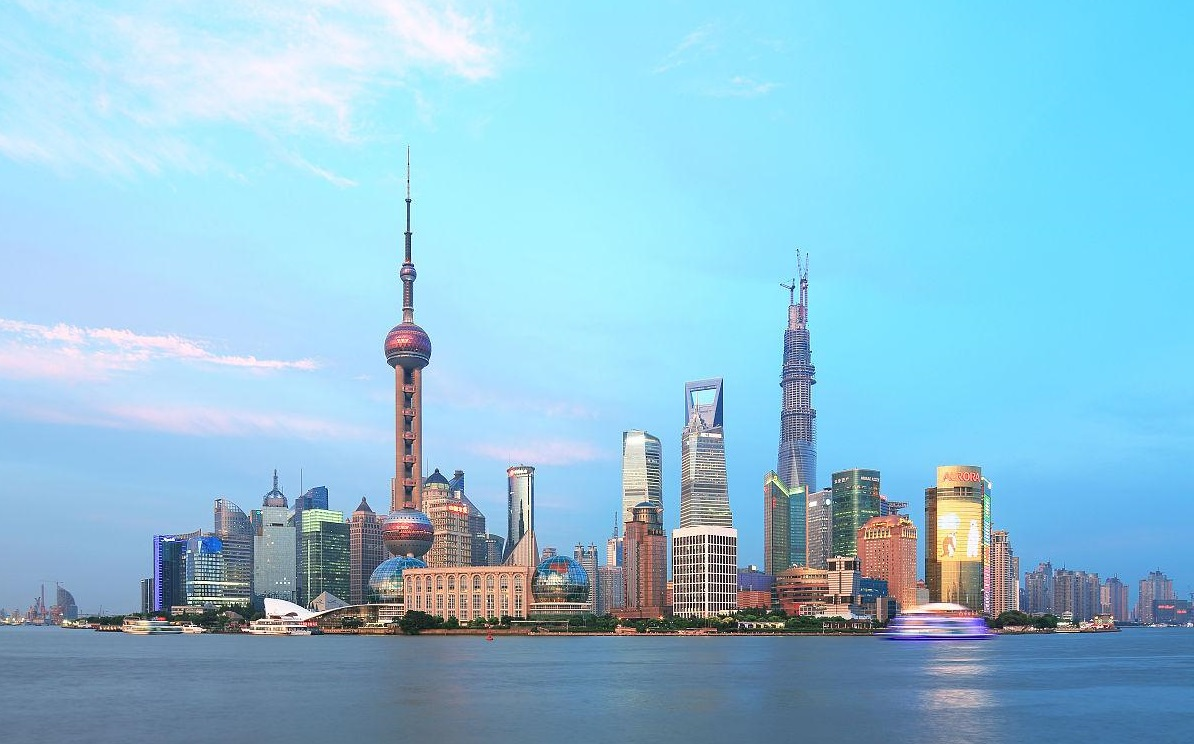
\includegraphics[width=0.6\textwidth]{figures/c1fig1.jpg}
	\caption{******}    
	\label{fig:fig07}
\end{figure}

\begin{figure}[h]
	\centering
	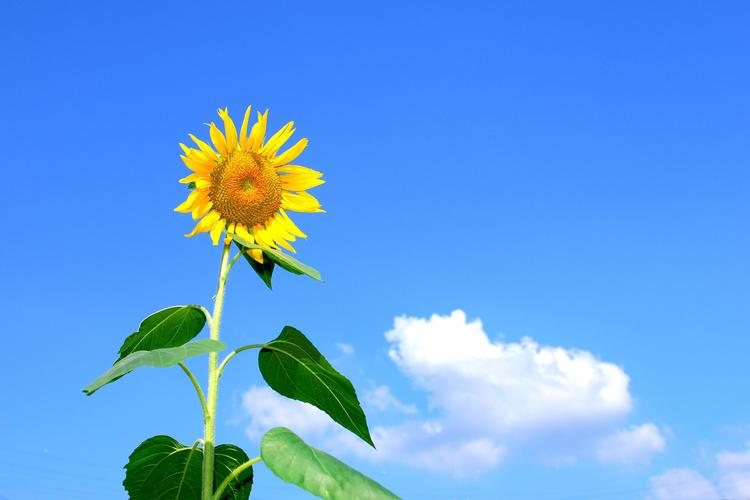
\includegraphics[width=0.6\textwidth]{figures/c1fig2.jpeg}
	\caption{******}    
	\label{fig:fig07}
\end{figure}

\section{国内外研究现状及发展趋势}
**********************




\section{论文主要内容和结构安排}
{\color{blue}河南师范大学}位于豫北名城新乡市，北依巍巍太行，南濒滔滔黄河，坐落在广袤的牧野大地、美丽的卫水之滨。学校是国家中西部高等教育振兴计划支持高校、国家“111计划”实施高校、河南省人民政府与教育部共建高校、教育部本科教学工作水平评估优秀学校和河南省特色骨干大学，\underline{河南省“双一流”创建高校}，三度蝉联全国文明单位，入选第二届全国文明校园{\color{red}\cite{R001}}。

文献{\color{red}\textcite{R002}}表明...............

\subsection{学校情况}
学校历史底蕴深厚，办学资源丰富\footnote{学校前身是始建于1923年的中州大学（原国立河南大学前身）理科和创建于1951年的平原师范学院，历经河南师范学院二院、河南第二师范学院、新乡师范学院等阶段，1985年始称河南师范大学。}。在百年的办学历程中，逐步熔铸了“厚德博学 止于至善”的校训、“明德 正学 倡和 出新”的校风、“修至学 立世范 启智慧 益品行”的教风、“尚诚朴 勤学问 重团结 养正气”的学风，积累和沉淀了“崇文明道 尚诚守德 抱朴求真”的师大精神，以校风淳、教风正、学风浓、教学水平高享誉省内外。学校占地面积139.53万平方米，建筑面积110.01万平方米，中外文纸质图书326.18余万册，电子图书1045.89余万册。建有全球唯一一家帕瓦罗蒂音乐艺术中心和河南省规模最大、种类最多的生物资源博物馆，办有附属中学、附属小学和幼儿园。

%%%   定理
\begin{thm}
	\rm{对于XXXXXXXXX，通过XXXXXXXXX可以表示为}
	\setlength\arraycolsep{1pt}   % 调整eqnarray等号两边空白
	\begin{eqnarray} 　 \label{eq3_06}   
		{{\pmb{\hat {\text g}}}_{mk}} = \sqrt {\tau {\rho _{\rm{\text p}}}} {{\pmb{\text R}}_{mk}}{{\pmb {\Xi }}_{mk}}{{\pmb{\mathord{\buildrel{\lower3pt\hbox{$\scriptscriptstyle\smile$}} \over {\text y}} }}_{mk,{\rm{\text p}}}},
	\end{eqnarray}
\end{thm}

%  证明
\begin{proof}
	根据XXXXXXXXXXX
\end{proof}

学校学科门类齐全，培养体系完备。现有哲学、经济学、法学、教育学、文学、历史学、理学、工学、农学、管理学、艺术学等11大学科门类。设有25个学院（部），4个书院，89个本科专业，其中国家一流本科专业建设点34个，省级一流本科专业建设点23个；32个硕士学位授权一级学科、21个硕士专业学位类别，10个博士学位授权一级学科、1个博士专业学位类别，7个博士后科研流动站，各类学生7.5万余人。拥有国家学科创新引智基地（“111计划”）2个、河南省特色骨干A类学科4个、河南省特需急需特色骨干学科（群）1个、河南省一级重点学科28个，化学、工程学、材料科学、环境/生态学、植物与动物科学等5个学科持续进入ESI全球前1\%，化学、地球与环境科学、物理学等3个学科持续进入本领域自然指数内地高校百强学科榜单。






\begin{table}
	\caption{\label{tab:test}不同DACs位数的量化系数} 
	\centering
	\renewcommand\arraystretch{1.2}  
	\begin{tabular}{c c c c c c}
		\hline
		{\kern 3pt}${b_m}$ & 1 & 2  & 3 & 4 &  5 {\kern 3pt}\\
		{\kern 3pt}${\alpha _m}$ & 0.6366 & 0.8825 & 0.96546 & 0.990503 &  0.997501 {\kern 3pt} \\
		\hline
	\end{tabular}
\end{table}








\chapter{标题标题标题标题标题标题}\label{chap:MIMOLP}
第二章内容第二章内容第二章内容第二章内容第二章内容
\section{标题1}
****************************
\subsection{子标题1}
****************************
\subsection{子标题2}
****************************

\section{标题2}
****************************
\section{标题3}
****************************

\section{本章小结}
****************************

\chapter{图神经网络辅助深度强化学习的非理想硬件去蜂窝大规模 MIMO 系统}\label{chap:MIMOLP}
在去蜂窝大规模多输入多输出（CF‑mMIMO）系统中，通过密集部署大量接入点（AP）可实现无缝通信覆盖，显著提升用户的频谱效率（SE）与系统总容量。然而，该方案的实施需要高昂的部署成本，且不可避免地需要采用非理想硬件。本章研究了在用户设备（UE）端使用非线性功率放大器（PA）、接入点端使用低精度模数转换器（ADC）的上行 CF‑mMIMO 系统中，用户可达速率的性能。

具体而言，本章推导了上行用户可达速率的闭合表达式，并综合分析了接入点数量、用户密度、接入点天线数以及 ADC 精度等多种因素的影响。为抑制用户间干扰并最大化和速率，本章提出一种基于图神经网络（GNN）辅助的演员‑评论家算法（DMAGNN‑AC）用于功率分配。所构建的框架克服了深度强化学习在高维非结构化状态空间中的表示瓶颈，并提供具有物理可解释性的特征嵌入。
与全功率发射方案相比，所提功率分配方案可使速率提升近一倍。此外，为缓解低精度 ADC 对速率的不利影响，本章进一步设计了一种增强型算法 —— 多智能体深度 Q 集成网络（MADQIN），以优化 ADC 精度的分配策略。最后，仿真结果验证了所提方案的有效性。
\section{引言}
在 CF‑mMIMO 系统中，随着接入点（AP）的大规模部署，硬件成本与功耗会随天线数量呈线性增长。一方面，采用低成本收发机替代高精度器件是一种可行的解决思路。然而在实际应用中，这类低成本方案会使射频（RF）链路更容易受到各类硬件损伤的影响。另一方面，采用低分辨率模数转换器（ADC）是实现低成本、低功耗 CF‑mMIMO 系统的有效途径，但该方式需要更为精准的信道模型与优化算法来抑制干扰与噪声。
为缓解硬件损伤带来的性能下降，通过优化功率分配以降低用户间干扰是一种有效的策略。传统优化算法如分数规划（FP）和加权最小均方误差（WMMSE）等，在理论层面可实现优异性能，但其过高的计算复杂度难以满足实际部署需求，且难以全面适配实际通信场景中的硬件损伤与信道衰落。相比之下，无模型机器学习方法，尤其是深度强化学习（DRL），凭借其较低的在线计算复杂度与无需先验训练数据集等优势，成为当前研究热点。然而，传统 DRL 难以有效捕捉用户间复杂的干扰关系与空间相关性，通常会导致优化效率偏低。

为突破这一局限，近期相关研究借助图表示方法建模多用户系统中的干扰关系与空间相关性。图神经网络（GNN）能够将原始信道状态信息（CSI）映射为低维图嵌入，显式保留用户间的空间关联特征，从而为 DRL 提供更具表征能力的状态空间。同时，GNN 对动态图结构（如用户移动带来的拓扑时变）的处理能力，与 DRL 的环境交互机制具有天然兼容性，二者深度融合可显著提升系统的移动性管理与网络协同性能。据此，本文提出一种高性价比、工程可实现的 CF‑mMIMO 通信方案，以充分挖掘系统性能潜力；并构建自适应网络优化框架，通过解耦功率分配问题，有效克服传统 DRL 在高维非结构化状态空间中存在的表示瓶颈。
\section{模型设计}
在本文中，我们考虑了一个如图 1 所示的上行链路 CF-mMIMO 系统，该系统由 MN 个天线的接入点（AP）和 K 个单天线的用户设备（UE）组成。所有接入点均通过回程链路与中央处理单元（CPU）相连。该系统采用时分双工（TDD）协议进行数据传输。由于本文仅关注上行数据传输阶段，因此相干时间间隔被分为两个阶段：1）上行链路训练；2）上行数据传输。
\subsection{信道估计}
在本研究中，我们采用了无相关瑞利衰落信道模型[25]。第 m 个接入点与第 k 个用户设备之间的信道增益被表示为

\begin{equation}\mathbf{g} _{mk} = {\beta _{mk}^{1/2} } {{\bf{h}}_{mk}},\end{equation}

它同时考虑了大规模衰落效应$\beta_{mk}$ 和小规模衰落 $\mathbf{h} _{mk}$ 。其中，$\beta_{mk}$ 同时考虑了几何衰减和阴影衰落，并且假定其在相干时间间隔内保持不变。$\mathbf{h} _{mk}$ 的元素是具有瑞利分布包络的复高斯随机变量。设 $\tau_\text{c}$ 为相干间隔的长度，$\tau_\text{p}$ 表示每个相干间隔的上行链路训练时间。由于训练时间长度的限制，我们采用 $\tau_\text{p} < K$ 的非正交导频，并将使用相同导频序列的 UE 集合定义为第 k 个 UE。在上行链路训练阶段，所有 K 个用户同时向所有 AP 发送非正交导频序列。第 k 个 UE 的导频信号可以表示为 $\sqrt{\tau_\text{p}}\boldsymbol{\varphi}_k\in \mathbb{C} ^{\tau_\text{p}\times1}$，其中 $\left\|\boldsymbol{\varphi}_k\right\|^2=1$ 。

本文采用更为精细的硬件非线性确定性行为模型，旨在更准确地建模导致硬件损伤的主要因素\cite{paper1}。该确定性行为模型的主要优势之一在于，其能够通过少量参数表征各类硬件损伤的物理效应。该模型将硬件输入–输出关系描述为\cite{paper2}
\begin{equation}
x_\text{out}=\sum_{i=0}^{N_p}a_{2i+1}x_\text{in}\left | x_\text{in} \right |^{2i}  
\end{equation}
式中，$a_{2i+1}$为模型复系数，非线性阶数可表示为$2N_p + 1$。该模型统一表征了功率放大器、本振、混频器及其他硬件器件的非线性特性。
需要指出的是，对于带内失真，由于偶次项主要出现在带外，准无记忆多项式中仅保留奇次项。此外，三次项能够刻画射频放大器中最主要的非线性来源 \cite {paper3},\cite {paper4}。因此，本文采用 的三次多项式模型。已有研究表明，三次多项式模型具有较高精度，可有效逼近功率放大器的实际非线性特性 \cite {paper5},\cite {paper6}。
经功率放大器非线性作用后，第 k个用户设备的输出信号可表示为
\begin{equation}
\label{eqn-1}\boldsymbol{\phi }_k = \underset{\tilde{a}_1 }{\underbrace{{a_1}\sqrt {{\tau _\text{p}}}} }  \boldsymbol{\varphi }_k + \underset{\tilde{a}_3 }{\underbrace{{a_3}{\tau _\text{p}}\sqrt {{\tau _\text{p}}}} }  \boldsymbol{\varphi} _k{\left\| {\boldsymbol{\varphi }_k} \right\|^2},
\end{equation}
式中，$\tilde{a}_1 \triangleq a_1\sqrt{\tau_\text{p}}$，$\tilde{a}_3 \triangleq a_3\tau_\text{p}\sqrt{\tau_\text{p}}$。第 $m$ 个接入点接收到的导频矩阵为
\begin{equation}\label{eqn-2}
\begin{aligned}
\mathbf{Y}_{\text{p},m} &= \sqrt {{\rho _\text{p}}}\sum_{k=1}^{K}  {{\bf{g}}_{mk}}\boldsymbol{\phi }_k^H + {\mathbf{W}_{\text{p},m}} \\
&= \sqrt {{\rho _\text{p}}}\sum_{k=1}^{K}  ({\tilde{a}_1}{{\bf{g}}_{mk}}\boldsymbol{\varphi} _k^H + \tilde{a}_3 {{\bf{g}}_{mk}}\boldsymbol{\varphi} _k^H{\left\| {\boldsymbol{\varphi }_k} \right\|^2}) + {\mathbf{W}_{\text{p},m}},
\end{aligned}
\end{equation}
式中，$\rho_\text{p}$ 为导频信号的归一化信噪比（SNR）。此外，$\mathbf{W}_{\text{p},m} \in \mathbb{C}^{N \times \tau_\text{p}}$ 表示第 $m$ 个接入点处的加性高斯白噪声（AWGN）矩阵，其第 $\varsigma$ 列满足分布
$\left [ \mathbf{W}_{\text{p},m} \right ] _\varsigma \sim \mathcal{CN} (\mathbf{0},\mathbf{I}_N)$。
本文采用非均匀量化器分析低精度模数转换器（ADC）对系统性能的影响。为此，引入经典的加性量化噪声模型（AQNM），该模型将量化过程引入的失真等效为高斯随机变量。已有研究验证，该模型在中低信噪比条件下具有足够的建模精度\cite{paper7},\cite{paper8}。结合式\eqref{eqn-2}，第 \(m\) 个接入点处ADC的输出可表示为
\begin{align}\label{eqn-3}{\tilde {\bf{Y}}_{\text{p},m}} & \triangleq {\alpha _m}{\mathbf{Y}_{\text{p},m}} + {\tilde {\bf{W}}_{\text{p},m}} \nonumber\\
&= {\alpha _m}\sqrt {{\rho _\text{p}}} \sum_{k=1}^{K}  ({\tilde{a} _1}{{\bf{g}}_{mk}}\boldsymbol{\varphi} _k^H + {\tilde{a}_3}{{\bf{g}}_{mk}}\boldsymbol{\varphi} _k^H{\left\| {\boldsymbol{\varphi}_k} \right\|^2})+ {\alpha _m}{\mathbf{W}_{\text{p},m}} + {\tilde{\bf{W}}_{\text{p},m}},\end{align}
式中，参数 $\alpha_m$ 决定第 $m$ 个接入点处模数转换器（ADC）的量化精度，且由量化比特数 $b_m$ 决定\cite{paper9}。此外，式\eqref{eqn-3}中的 $\tilde{\mathbf{W}}_{\text{p},m}$ 表示第 $m$ 个接入点处的加性高斯量化噪声，该噪声与 $\mathbf{Y}_{\text{p},m}$ 互不相关，其协方差矩阵可表示为
\begin{align}\label{eqn-4}
\mathbf{R}_{\tilde{ \mathbf{W}}_{\text{p},m}} &= \mathbb{E}\left\{ {{\tilde{\mathbf{W}}_{\text{p},m}}\tilde {\mathbf{W}}_{\text{p},m}^H} \right\} \nonumber\\ 
&= {\alpha _m}(1 - {\alpha _m})\text{diag}\left(\mathbb{E}\left\{ {{\mathbf{Y}_{\text{p},m}}\mathbf{Y}_{\text{p},m}^H} \right\} \right). 
\end{align}
在第 \(m\) 个接入点对接收导频信号完成量化后，将量化信号 \(\tilde{\mathbf{Y}}_{\text{p},m}\) 向 \(\boldsymbol{\varphi}_k\) 投影可得
\begin{align}\label{eqn-5}
\check{\mathbf{y} }_{\text{p},mk}&\triangleq {\tilde{\mathbf{Y}}_{\text{p},m}}\boldsymbol{\varphi }_k \nonumber\\
%&= {\alpha _m}\sqrt {{\rho _p}} \mathop \sum \nolimits_{k' = 1}^K ({b_1}{{\bf{g}}_{mk'}}\varphi _{k'}^H + {b_3}{{\bf{g}}_{mk'}}\varphi _{k'}^H{\left| {{\varphi _{k'}}} \right|^2}){\varphi _k} + {\alpha _m}{W_{p,m}}{\varphi _k} + {{\tilde W}_{p,m}}{\varphi _k}\\
&= {\alpha _m}\sqrt {{\rho _\text{p}}}\sum_{k'\in \mathcal{P}_k }^{K}  ({\tilde{a}_1} + {\tilde{a}_3}\tau_\text{p}){{\bf{g}}_{mk}}\nonumber \\
&\quad + {\alpha _m}{\mathbf{W}_{\text{p},m}}\boldsymbol{\varphi}_k + {{\tilde{\mathbf{W}}}_{\text{p},m}}\boldsymbol{\varphi}_k.
\end{align}
基于上述推导，可得如下引理。
引理：
采用最小均方误差（MMSE）方法得到的信道向量 $\mathbf{g}_{mk}$ 估计值可表示为
\begin{equation}\label{eqn-6}
\mathbf{\hat{g} }_{mk} = c_{mk} \mathbf{\check{y} }_{\text{p},mk},
\end{equation}
其中
\begin{align}\label{eqn-7}
{c_{mk}} &= \mathbb{E}\left \{ \mathbf{g}_{mk}^H\mathbf{\check{y} }_{\text{p},mk}   \right \} \left ( \mathbb{E}\left \{  \mathbf{\check{y} }_{\text{p},mk}^H\mathbf{\check{y} }_{\text{p},mk}\right \}   \right )^{-1}   \nonumber \\
%&= \frac{{\sqrt {{\tau _p}{\rho _p}} N{\beta _{mk}}{\alpha _m}({a_1} + {a_3}{\tau _p})}}{{N{\alpha _m}({\tau _p}{\rho _p}({a_1} + {a_3}{\tau _p}){\beta _{mk}} + 1)}}{{\bf{\mathord{\buildrel{\lower3pt\hbox{$\scriptscriptstyle\smile$}} \over y} }}_{p,mk}} \\%
&= \frac{{\sqrt {{\tau _\text{p}}{\rho _\text{p}}} {\beta _{mk}}({a _1} + {a _3}{\tau _\text{p}})}}{{{\tau _\text{p}}{\rho _\text{p}}\sum_{k'\in \mathcal{P}_k }^{K} ({a _1} + {a _3}{\tau _\text{p}})^2{\beta _{mk}} + 1}}.
\end{align}
将信道估计第 \(n\) 个分量的均方值记为
\begin{align}\label{eqn-8}
\gamma_{m k}&=\mathbb{E}\left \{ \left | \left [ \mathbf{\hat{g} }_{mk}  \right ]_n  \right |^2  \right \}\nonumber \\ &=\frac{\tau_\text{p} \rho_\text{p} \alpha_{m} \beta_{m k}^{2}\left(a_{1}+a_{3} \tau_\text{p}\right)^{2}}{\tau_\text{p} \rho_\text{p}\sum_{k'\in \mathcal{P}_k }^{K} \left(a_{1}+a_{3} \tau_\text{p}\right)^2 \beta_{m k}+1}.
\end{align}
令 $\boldsymbol{\tilde{g}}_{mk} = \mathbf{g}_{mk} - \hat{\mathbf{g}}_{mk}$ 为信道估计误差。根据线性最小均方误差（MMSE）估计的性质，$\boldsymbol{\tilde{g}}_{mk}$ 与 $\hat{\mathbf{g}}_{mk}$ 相互独立且服从复高斯分布。因此，信道估计误差向量 $\boldsymbol{\tilde{g}}_{mk}$ 中各元素的均方误差满足
$\left[\boldsymbol{\tilde{g}}_{mk}\right]_n \sim \mathcal{CN}\!\left( 0, \beta_{mk}-\gamma_{mk} \right)$。
\subsection{上行数据传输}
在上行数据传输阶段，所有用户设备（UE）同时向接入点（AP）发送数据 $q_k$，其中满足 $\mathbb{E}\{|q_k|^2\}=1,\forall k$。经用户设备侧功率放大器（PA）的非线性作用后，第 $k$ 个用户设备的输出信号为
\begin{align}
\label{eqn-9}{y_k} &= \sqrt {{\rho _\text{u}}} \left( {{a_1}\sqrt {{\eta _k}} {q_k} + {a_3}\sqrt {{\eta _k}} {q_k}{{\left| {\sqrt {{\eta _k}} {q_k}} \right|}^2}} \right)\nonumber \\ 
&= \sqrt {{\rho _\text{u}}} \left( {{\tilde{a}_{1k}}{q_k} + {\tilde{a}_{3k}}{q_k}{{\left| {{q_k}} \right|}^2}} \right),
\end{align}
式中，$\rho_\text{u}$ 表示各用户设备的最大归一化发射功率，$\tilde{a}_{1k} \triangleq a_1\sqrt{\eta_k}$，$\tilde{a}_{3k} \triangleq a_3\eta_k\sqrt{\eta_k}$。此外，功率控制系数 $\eta_k$（$\forall k$）的选取需满足 $\mathbb{E}\left\{|y_k|^2\right\} \le \rho_\text{u}$。因此，该约束可简化为
\begin{equation}\label{eqn-10}
{\left| {{a_1}} \right|^2}{\eta _k} + 2(a_1^ * {a_3} + {a_1}a_3^ * )\eta _k^2 + 6{\left| {{a_3}} \right|^2}\eta _k^3 \le 1,  \forall k.
\end{equation}
第 \(m\) 个接入点接收到的复基带信号可表示为
\begin{equation}\label{eqn-11}
{{\bf{y}}_{\text{u},m}} = \sqrt {{\rho _\text{u}}} \sum_{k = 1}^K ({\tilde{a}_{1k}}{{\bf{g}}_{mk}}{q_k} + {\tilde{a}_{3k}}{{\bf{g}}_{mk}}{q_k}{\left| {{q_k}} \right|^2}) + {\bf{w}}_{\text{u},m},
\end{equation}
式中，$\mathbf{w}_{\text{u},m}\sim \mathcal{CN}(\mathbf{0},\mathbf{I}_N)$ 表示加性噪声。随后，第 \(m\) 个接入点的接收信号经ADC量化，其量化输出可表示为
\begin{align}\label{eqn-12}{{\bf{\tilde y}}_{\text{u},m}} &= {\alpha _m}{{\bf{y}}_{\text{u},m}} + {{\bf{\tilde w}}_{\text{u},m}} \nonumber\\
&= {\alpha _m}\sqrt {{\rho _\text{u}}} \sum_{k = 1}^K ({\tilde{a}_{1k}}{{\bf{g}}_{mk}}{q_k} + {\tilde{a}_{3k}}{{\bf{g}}_{mk}}{q_k}{\left| {{q_k}} \right|^2}) \nonumber\\
&\quad+ {\alpha _m}{{\bf{w}}_{\text{u},m}} + {{\bf{\tilde w}}_{\text{u},m}},
\end{align}
式中，$\boldsymbol{\tilde w}_{\text{u},m}$ 表示量化噪声，其协方差矩阵可表示为
\begin{align}{\mathbf{R}_{{{{\bf{\tilde w}}}_{\text{u},m}}}} \approx {\alpha _m}(1 - {\alpha _m})\text{diag}(\mathbb{E}\left\{ {{{\bf{y}}_{\text{u},m}}{\bf{y}}_{\text{u},m}^H} \right\}).\end{align}
为检测 $q_k$，各接入点（AP）采用分布式方式，通过低复杂度的匹配滤波合并计算本地数据估计值，随后经前传链路将信号汇总至中央处理单元（CPU）进行聚合与译码。由此，中央处理单元处的接收信号可表示为
\begin{align}\label{eqn-14}
{r_{\text{u},k}} &= \sum_{m = 1}^M {\bf{\hat{g}}}_{mk}^H{{{\bf{\tilde y}}}_{\text{u},m}}\nonumber\\
& = \sqrt {{\rho _\text{u}}}  \sum_{m = 1}^M {\alpha _m}\sum_{k' = 1}^K {\bf{\hat g}}_{mk}^H{\tilde{a}_{1k'}}{{\bf{g}}_{mk'}}q_{k'}  
\nonumber\\& \quad+ \sqrt {{\rho _\text{u}}} \sum_{m = 1}^M {\alpha _m}\sum_{k' = 1}^K {\bf{\hat g}}_{mk}^H{\tilde{a}_{3k'}}{{\bf{g}}_{mk'}}q_{k'} {\left| {q_{k'} } \right|^2}
 \nonumber\\& \quad+ \sum_{m = 1}^M {\bf{\hat g}}_{mk}^H{\alpha _m}{{\bf{w}}_{\text{u},m}} + \sum_{m = 1}^M {{{\bf{\hat g}}}^H_{mk}}{{{\bf{\tilde w}}}_{\text{u},m}}.
\end{align}	
随后，基于 $r_{\text{u},k}$ 对 $q_k$ 进行检测。在下一节中，我们将推导可达速率的闭式表达式。
\subsection{可实现速率分析}
本节在同时考虑功率放大器（PA）非线性与低精度模数转换器（ADC）的条件下，推导了CF-mMIMO系统中上行用户设备的可达速率。由于各接入点仅能获取信道估计信息，中央处理单元（CPU）无法获知真实信道状态。尽管中央处理单元未知当前实际信道状态，但其假设信道状态的均值已知，并利用该已知均值计算可达速率\cite{paper6}。结合式\eqref{eqn-14}，可将中央处理单元的接收信号重新表示为
\begin{align}\label{eqn-15}
{r_{\text{u},k}}& = {\text{ES}_k} \cdot {q_k} + {\text{BU}_k} \cdot {q_k} + \sum_{k' \ne k}^K {\text{I}_{kk'}} \cdot q_{k^\prime} \nonumber \\
&\quad+\sum_{k' \ne k}^K {\text{NB}_{kk'}} \cdot q_{k^\prime}  + {\text{N}_k} + {\text{Q}_k},
\end{align}
式中，$\text{ES}_k$、$\text{BU}_k$、$\text{I}_{kk'}$、$\text{NB}_{kk'}$、$\text{N}_k$ 和 $\text{Q}_k$ 分别表示第 \(k\) 个用户设备的期望信号确定性分量、波束成形不确定性、第 \(k'\) 个用户设备产生的干扰、第 \(k\) 个用户设备功率放大器非线性引入的干扰、加性噪声以及量化噪声，其具体表达式为
\begin{equation}\label{eqn-16}
{\text{ES}_k} = \sqrt {{\rho _\text{u}}} \mathbb{E}\left\{ {\sum_{m = 1}^M {\alpha _m}\left({\tilde{a} _{1k}}{\bf{\hat g}}_{mk}^H{{\bf{g}}_{mk}} + {\tilde{a} _{3k}}{\bf{\hat g}}_{mk}^H{{\bf{g}}_{mk}}{{\left| {{q_k}} \right|}^2}\right)} \right\},
\end{equation}
\begin{equation}\label{eqn-17}
\begin{aligned}{\text{BU}_k} &= \sum_{m = 1}^M \alpha_m \sqrt{\rho _\text{u}}\left({\tilde{a} _{1k}}{\bf{\hat g}}_{mk}^H{{\bf{g}}_{mk}} + {\tilde{a} _{3k}}{\bf{\hat g}}_{mk}^H{{\bf{g}}_{mk}}{\left| {{q_k}} \right|^2}\right)\\ 
&- \mathbb{E} \left\{ {\sum_{m = 1}^M {\alpha _m}\sqrt{\rho _\text{u}}\left({\tilde{a} _{1k}}{\bf{\hat g}}_{mk}^H{{\bf{g}}_{mk}} + {\tilde{a} _{3k}}{\bf{\hat g}}_{mk}^H{{\bf{g}}_{mk}}{{\left| {{q_k}} \right|}^2}\right)} \right\},
\end{aligned}\end{equation}
\begin{equation}\label{eqn-18}{\text{I}_{kk'}} = \sqrt {{\rho _\text{u}}}\sum_{m = 1}^M {\alpha _m}{\tilde{a}_{1k'}}{{\bf{\hat g}}^H_{mk}}{{\bf{g}}_{mk'}},\end{equation}
\begin{equation}\label{eqn-19}{\text{NB}_{kk'}} = \sqrt {{\rho _\text{u}}} \sum_{m = 1}^M {\alpha _m}{\tilde{a}_{3k'}}{{\bf{\hat g}}^H_{mk}}{{\bf{g}}_{mk'}}{\left| {{q_{k'}}} \right|^2},\end{equation}
\begin{equation}\label{eqn-20}{\text{N}_k} = \sum_{m = 1}^M {\alpha _m}{\bf{\hat g}}_{mk}^H{{\bf{w}}_{\text{u},m}},\end{equation}
\begin{equation}\label{eqn-21}{\text{Q}_k} = \sum_{m = 1}^M {{\bf{\hat g}}^H_{mk}}{{\bf{\tilde w}}_{\text{u},m}}.\end{equation}
将式\eqref{eqn-15}中干扰与噪声之和等效为有效噪声。在最坏情况下，将干扰项视为不相关高斯噪声随机变量，由此可得第 \(k\) 个用户的上行可达速率如式\eqref{eqn-22}所示。

定理1：
在具有协整波束成形（CB）的CF‑mMIMO系统中，对于任意有限的 \(M\) 和 \(K\)，第 \(k\) 个用户设备的可达速率由式\eqref{eqn-23}给出（见下页顶部）。
\begin{figure*}[ht]
	\centering
	\begin{equation}\label{eqn-22}
		{R_{\text{u},k}}= {\log _2}\left(1 + \frac{{{{\left| {{\text{ES}_k}} \right|}^2}}}{{\mathbb{E}\left \{\left |  \text{BU}_k \right | ^2 \right \}   +\sum \limits_{k'\ne k}^{K} \mathbb{E} \left \{ \left | \text{I}_{kk'} \right |^2  \right \}   +  \sum \limits_{k'\ne k}^{K}\mathbb{E}\left \{ \left |  {\text{NB}_{kk'}}  \right |^2  \right \}  +\mathbb{E} \left \{ \left | {\text{N}_k} \right |^2  \right \}   +  \mathbb{E}\left \{ \left |  \text{Q}_k\right | ^2 \right \}  } }\right).
	\end{equation}
	\hrulefill
	\begin{equation}\label{eqn-23}
		R_{\text{u}, k}=\log _{2}\left(1+\frac{N^{2} \rho_\text{u}\left|\tilde{a}_{1 k}+\tilde{a}_{3 k}\right|^{2}\left(\sum\limits_{m=1}^{M} \alpha_{m} \gamma_{m k}\right)^{2}}{N^{2} \rho_\text{u} \sum\limits_{k'=1}^{K}\left(\Omega_{k^{\prime}} \sum\limits_{m=1}^{M} \alpha_{m}^{2} \gamma_{m k} \beta_{m k'}\right)+3 N^{2} \rho_\text{u}\left|a_{3}\right|^{2} \eta_{k}^{3}\left(\sum\limits_{m=1}^{M} \alpha_{m}^{2} \gamma_{m k}\right)^{2}+N^{2} \sum\limits_{m=1}^{M} \alpha_{m}^{2} \gamma_{m k}+\Psi _k }\right),
	\end{equation}
	\flushleft{where}
	\begin{equation}\begin{aligned}\Omega _k = \left( {{{\left| {{a_1}} \right|}^2}{\eta _{k}} + 2a_1^*{a_3}{\eta _{k}^2}+ 2{a_1}a_3^ * \eta _{k}^2 + 6{{\left| {{a_3}} \right|}^2}\eta _{k}^3} \right), \end{aligned}\end{equation}
	\begin{equation}\Psi _k={N}{\rho _\text{u}}\mathop \sum \limits_{m = 1}^M {\alpha _m}(1 - {\alpha _m})\left( {\mathop \sum \limits_{k = 1}^K {\beta _{mk}}\Omega _k + 1} \right){\gamma _{mk}}.\end{equation}
	\hrulefill
\end{figure*}
基于式\eqref{eqn-23}，我们对配备**非线性功率放大器（PA）和低精度模数转换器（ADC）** 的小区-free 大规模MIMO（CF-mMIMO）系统性能，给出以下几点关键分析与见解。

定理1推导了可达速率的精确闭式表达式，清晰揭示了关键参数与系统性能之间的内在关联。具体而言，式(23)中的系数 \(a_3\) 表征功率放大器的非线性特性。随着功率放大器非线性程度的增强，\(a_3\) 的绝对值呈增大趋势。这一变化会使信干噪比的分子减小、分母增大，进而导致用户速率显著下降。这表明功率放大器的非线性对用户速率存在明显的负面影响。

此外，从表达式分子与分母的构成可以看出，除量化噪声项外，其余各项均包含 \(N\) 的平方因子。将分子与分母同除以 \(N^2\) 后可以发现，仅有项
${\rho _\text{u}}\mathop \sum \limits_{m = 1}^M {\alpha _m}(1 - {\alpha _m})\left( {\mathop \sum \limits_{k = 1}^K {\beta _{mk}}\Omega _k + 1} \right){\gamma _{mk}}/N$与 \(N\) 相关。随着 \(N\) 逐渐增大，用户速率在初始阶段会有一定程度的提升；当 \(N\) 相对于${\rho _\text{u}}\mathop \sum \limits_{m = 1}^M {\alpha _m}(1 - {\alpha _m})\left( {\mathop \sum \limits_{k = 1}^K {\beta _{mk}}\Omega _k + 1} \right){\gamma _{mk}}$足够大时，其对可达速率的影响将渐近趋近于零。

\section{上行和速率最大化}
由于各接入点会接收所有用户设备发送的信号，用户间干扰会导致目标用户的速率显著下降。因此，调控其他用户的发射功率，以平衡目标信号与干扰信号之间的关系，具有重要意义。

基于上述背景及闭式解中的可调变量参数，本节构建上行功率控制模型。该模型以非负功率集合为约束前提，目标是最大化系统总速率，且优化过程需满足系统功率约束条件，即每个变量均不超过预设的最大功率限值。根据式\eqref{eqn-23}，上行总速率最大化问题的数学表达式为
\begin{align} \label{P1}
\mathcal{P}_1:& \quad \underset{\left \{ \eta _k \right \} }{\text{max}} \quad  {\sum_{k=1}^{K}} R_{\text{u},k}\\
\text{s.t.}&\quad {\left| {{a_1}} \right|^2}{\eta _k} + 2(a_1^ * {a_3} + {a_1}a_3^ * )\eta _k^2 + 6{\left| {{a_3}} \right|^2}\eta _k^3 \le 1, \forall k.
\end{align}
通常情况下，优化问题 $\mathcal{P}_1$ 属于非凸NP‑难问题。该特性使得基于模型的方法既无法精确量化其与最优解之间的性能差距，也会带来较高的计算复杂度。此外，基于模型的方法自适应能力有限，难以灵活适配未来异构业务需求的多样性与环境的随机变化。值得注意的是，信道状态信息 $\mathbf{g}_{mk}$ 是求解该问题的关键统计量，其中蕴含了用于确定最优功率控制方案的重要信息。因此，$\mathbf{g}_{mk}$ 与对应功率控制系数 $\eta_k$ 之间潜在存在某种映射关系。针对上述挑战，本文采用数据驱动的深度强化学习（DRL）算法来挖掘并实现这一映射关系。

此外，基于式\eqref{eqn-23}的推导结果可知，用户速率随ADC量化系数 $\alpha_m$ 的增大呈单调递增趋势。结合量化噪声项的影响，可通过动态调整ADC量化比特数实现系统总速率最大化。为此，本文采用改进型深度Q学习算法作为优化手段，以用户总速率最大化为目标，将ADC量化精度分配问题正式表述为
\begin{align}\label{P2}
\mathcal{P}_2 :&\quad\underset{\left \{ b_m \right \} }{\text{max}} \quad  {\sum_{k=1}^{K}} R_{\text{u},k}\\
\text{s.t.}&\quad   b_m=0,1,2,...,  \forall m, \\
\quad & \quad N\sum_{m=1}^{M} b_m=B_\text{\text{max}},
\end{align}
式中，$B_\text{max}$ 为所有接入点（AP）上模数转换器（ADC）的固定总量化比特数。

基于上述两类优化问题，本文将在后续两节中分别采用两种算法，对CF‑mMIMO系统的性能进行分析与探究。

\section{DMAGNN-AC算法设计}

在深度强化学习中，马尔可夫决策过程（MDP）是对序贯决策问题进行建模的核心框架。通常在MDP问题中，存在一个或多个智能体与环境进行交互。智能体根据策略函数$\pi$与当前状态$s$选择并执行动作$a$，环境以奖励$r$的形式给出反馈，用于评估动作$a$的优劣，并转移至下一状态$s'$。在一个完整回合中，智能体会进行多次此类动作选择，这些动作与状态转移共同构成由元组$(\mathcal{S},\mathcal{A},\mathcal{P},\mathcal{R})$所描述的马尔可夫决策过程。其中，$\mathcal{S}$为状态空间，$\mathcal{A}$为动作空间，$\mathcal{P}$为状态转移概率函数，表示在状态$s$下执行动作$a$后转移至状态$s'$的概率，$\mathcal{R}$为奖励函数，定义在状态$s$下执行动作$a$后的期望回报。

为利用深度强化学习算法实现功率分配，本文将优化问题$\mathcal{P}_1$建模为马尔可夫决策过程。然而，由于用户间存在复杂的干扰关系与空间相关性，传统深度强化学习难以有效学习到最优策略。针对该问题，本文设计一种动态多智能体图神经网络（DMAGNN）框架，用于提取用户间的干扰特征，提供结构化的状态信息，从而有效提升深度强化学习的性能。在该框架中，中央处理单元（CPU）作为智能体，环境由用户设备、接入点等组件构成。所提DMAGNN将用户与接入点之间的信道状态信息建模为节点特征，将不同用户间的干扰建模为边。该神经网络的详细设置与具体流程如图fig2所示（见本页顶部）。

\begin{figure}
\centering
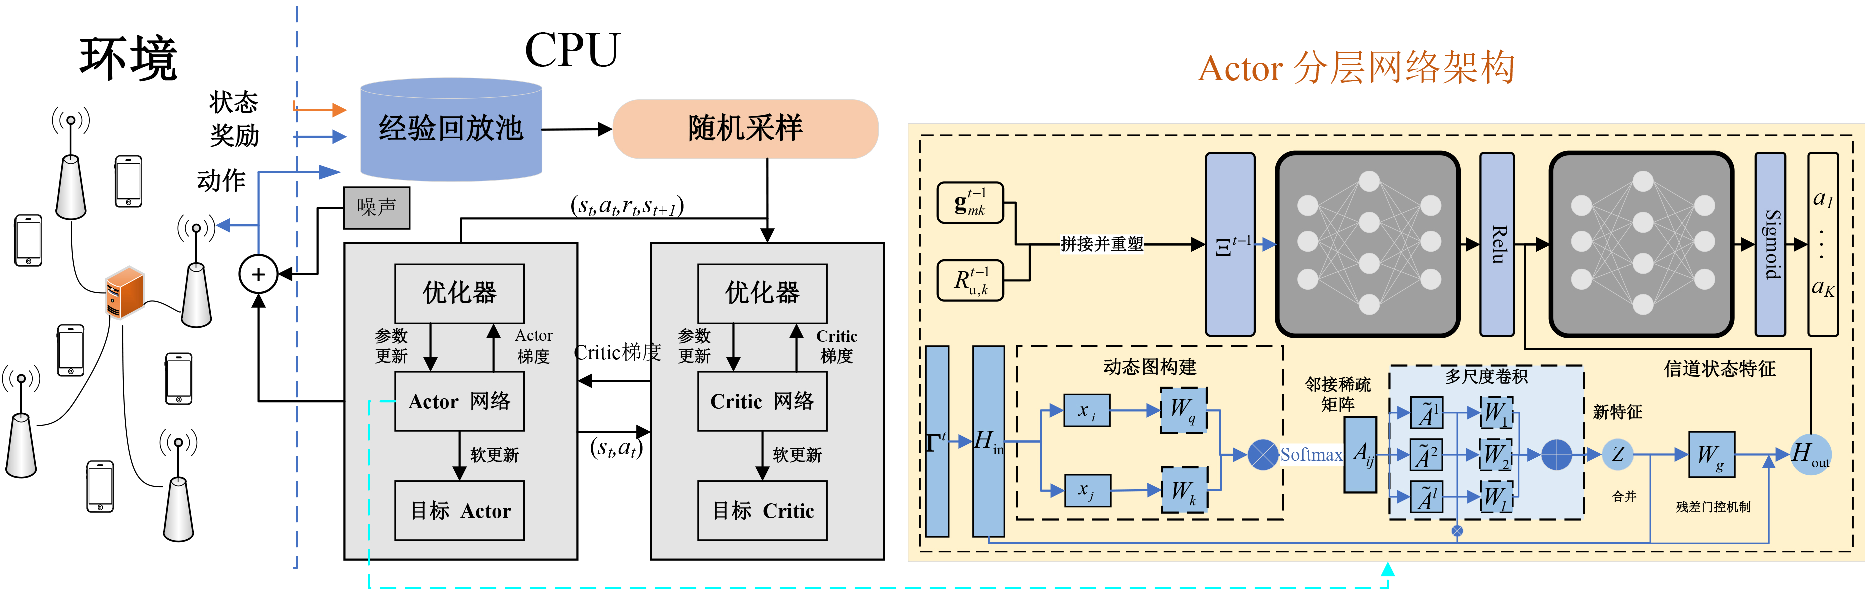
\includegraphics[width=5in] {fig2}
\caption{DMAGNN-AC网络架构图。}
\label{fig2}
\end{figure}

\subsection{DMAGNN-AC 组件}
$\emph{1) 状态}$：本文在第三节中指出，第 \(k\) 个用户设备与第 \(m\) 个接入点之间的信道状态信息 \(\mathbf{g}_{mk}\) 到第 \(k\) 个用户设备功率控制系数 \(\eta_k\) 之间存在某种映射函数。但由于中央处理单元（CPU）无法获取信道实时观测值，本文最终采用理论信道状态信息 \(\mathbf{g}_{mk}\) 作为神经网络的输入。因此，神经网络的输入可表示为
\begin{equation}\mathbf{\Gamma}^t:=\left \{  \mathbf{g}_{mk}^t  \mid \forall m,k\right \}.	\end{equation} 

然而，考虑到训练过程本质上是与时间序列紧密相关的马尔可夫过程，直接将变量 $\mathbf{\Gamma}^t$ 作为神经网络的输入并不合理。同时，在指定时间跨度内，用户移动行为引发的环境状态变化可被视为一个时间序列演化过程；在该演化过程中，用户在时空维度的移动特征是预测其下一时刻行为的关键依据。

为此，本文引入时刻 $(t-1)$ 下的 $\mathbf{g}_{mk}$ 与 $R_{\text{u},k}$ 作为神经网络输入的辅助信息，使其与 $\mathbf{\Gamma}^t$ 共同参与下一时刻动作的预测。辅助信息的具体定义为
\begin{equation}\mathbf{\Xi} ^{t-1}:=\left \{\mathbf{g}_{mk}^{t-1} , R_{\text{u},k}^{t-1} \mid \forall m,k \right \}  .\end{equation} 
神经网络的最终输入可表示为
\begin{equation}s^{t}:=\left \{ \mathbf{\Xi} ^{t-1}, \mathbf{\Gamma} ^t\right \}. \end{equation}
此时，状态空间的基数为$2 \left ( MK \right ) +K$。

$\emph{2) 动作}$：演员网络根据当前状态 \(s\) 进行决策，输出 \(K\) 个用户设备的上行发射功率系数，可表示为
\begin{equation}a ^{t}=\left [ \eta _1^{t},...,\eta _K^{t} \right ] ,\end{equation}

式中，$\eta _k^{t}$满足约束条件 $0\le \eta _k^{t}\le \eta _\text{max}, \forall k$。

\emph{3) 奖励}：本文直接以实际获得的用户速率作为环境反馈的奖励函数，其定义为
\begin{equation}r^{t+1} = \textstyle \sum_{k=1}^{K} R_{\text{u},k}^{t}.\end{equation}

\subsection{算法设计}
所提算法的具体设计体现在以下四个方面。
\subsubsection{Actor 网络分层设计}
本文将 Actor 网络设计为分层结构，旨在合理划分功能并有效融合信息。具体而言，上层网络主要对信息 $\mathbf{\Xi }^{t-1}$ 进行特征提取与融合；随后，将上层网络的输出与信息 $\mathbf{\Gamma} ^t$ 的特征相结合，作为下层网络的输入。下层网络的核心功能是基于上述融合特征完成动作预测。

在将 $\mathbf{\Gamma} ^t$ 输入至下层网络之前，本文采用自主设计的DMAGNN对 $\mathbf{\Gamma} ^t$ 进行特征提取。DMAGNN的运行流程包含以下步骤：
\begin{itemize}
\item {\bf{节点特征初始化：}}
第 \(k\) 个用户设备在 \(t\) 时刻的节点特征被初始化为
\begin{equation}\label{eq-38}x_k=\text{vec}(H_{\text{in},k}^HH_{\text{in},k})\in \mathbb{R}^d, \end{equation}
式中，$H_{\text{in},k}\in \mathbb{C} ^{M\times N}$ 表示第 \(k\) 个用户设备到 \(M\) 个接入点（AP）的信道矩阵。

\item{\bf{动态图结构学习}}
在图构建过程中，传统图结构通常依靠固定的地理距离（如路径损耗）来定义节点间的连接关系。然而在CF‑mMIMO系统中，用户设备分布密集、干扰特性复杂，固定图结构无法反映瞬时信道状态带来的影响。为此，本文借鉴图注意力网络（GAT）的注意力机制，引入可学习的参数化距离度量，并利用双线性注意力机制计算节点 \(i\) 与节点 \(j\) 之间的关联强度。
\begin{equation}\label{eq-39}a_{ij}=\sigma \left ( \frac{\left ( W_qx_i \right ) \cdot \left ( W_kx_j \right )  ^T}{\sqrt{b} } \right  ), \end{equation}
式中，$b$ 为缩放因子，$W_q$ 和 $W_k$ 是可训练的投影矩阵，用于将节点特征 $x_i$、$x_j$ 分别映射到查询空间与键空间。
查询空间用于表示当前节点（如用户 $i$）的查询特征，键空间则用于表示其他节点（如用户 $j$）的被查询特征。
通过计算二者的内积，可以衡量两个节点之间的关联程度与相似度。该机制使模型能够动态学习节点间的关联关系，而非依赖预先定义的图结构。

{\emph{定理 2:}} 为降低全连接图 $O(K^2)$ 的计算复杂度，本文设计了稀疏邻接矩阵形式。
\begin{equation}\label{eq-40}A_{ij}=\left\{\begin{matrix}
  1,& \text{if} \hspace{0.1cm} a_{ij}> \vartheta \hspace{0.1cm} \text{and}\hspace{0.1cm} i\ne j\\ 
  0,& \text{otherwise},
\end{matrix}\right.\end{equation}
式中，动态阈值 $\vartheta$ 通过自适应二分搜索确定，以保证非零边的数量满足 $\left | E \right | =O\left ( K\log K \right )$。
通过对邻接矩阵进行稀疏化处理，模型仅保留相关性较强的连接，从而提升泛化性能。

\item{\bf{多尺度特征聚合：}}
多尺度卷积通过聚合不同范围的邻域信息，增强模型对复杂空间相关性的捕获能力，从而解决传统单层图卷积网络（GCN）感受野有限的问题。多跳信息聚合公式可表示为
\begin{equation}\label{eq-41}\text{GCN}\left ( A,H_{\text{in}} \right ) =\sum_{l=0}^{L} \tilde{A} ^lH_{\text{in}}W_l,\end{equation}
式中，$\tilde{A} =D^{-\frac{1}{2}}AD^{-\frac{1}{2}}$ 为邻接矩阵 $A$ 的对称归一化形式，$D=\text{diag}\left(\sum_j A_{1j},\dots,\sum_j A_{Kj}\right)$ 为度矩阵，$W_l\in\mathbb{R}^{d\times d}$ 为第 $l$ 跳对应的可训练权重矩阵。该设计具备以下特点：
\begin{itemize}
    \item 局部性保持：当 \(l=0\) 时，保留节点自身特征。
    \item 邻域扩展：$l=1$ 时聚合一阶邻域信息，$l=2$ 时捕获二阶邻域信息。
\end{itemize}
同时，为不同跳数设置独立的 $W_l$，以避免特征混淆。

\item{\bf{门控特征更新机制：}}
最后，本文采用门控机制实现节点特征的选择性更新，具体过程可表示为
\begin{equation}\label{eq-42}Z=\text{GCN}\left ( A,H_{\text{in}} \right ), \end{equation}
\begin{equation}\label{eq-43}G=\sigma \left ( W_g\left [ H_{\text{in}}  \oplus Z \right ]  \right ),\end{equation}
\begin{equation}\label{eq-44}H_{\text{out}}=\text{LayerNorm}\left ( G\odot H_{\text{in}}+\left ( 1-G \right ) \odot Z \right ), \end{equation}
式中，$Z$ 为卷积后生成的新特征，$W_g\in\mathbb{R}^{2d\times d}$ 为门控权重矩阵。
门控机制可动态选择保留原始特征 $H_{\text{in}}$ 与新特征 $Z$ 的比例，从而缓解梯度消失问题。
\end{itemize}

\begin{algorithm}[t]
    \renewcommand{\algorithmicrequire}{\textbf{输入:}}
    \renewcommand{\algorithmicensure}{\textbf{输出:}}
    \caption{DMAGNN-AC 功率分配算法}
    \label{DDPG}
    \begin{algorithmic}[1]
    			\State $\emph{输入：}$ 回合次数 $T_e$， 探索次数 $T$， 折扣因子 $\gamma$， 学习率 $\alpha$， 随机数据量 $R_q$， 批次大小 $\mathcal{N}$， 神经网络更新权重 $\tau$。 % input
    			
    			\State $\emph{初始化：}$ 采用 He 初始化方法\footnotemark[1]初始化Critic网络 $C(s,a;\omega _c)$、Actor网络 $A(s;\omega _a)$ 的参数 $\omega _c$ 和 $\omega _a$，并且初始化 DMAGNN 的参数与初始状态 $s^1$。

        \For {$k=1$ to $T_e$}
        		\State 设置环境变量初始值。
        		
	        \For {$\jmath =1$ to $T$}
	        		\State 二分搜索阈值 $\vartheta$.
	            
		        \If {$\jmath < R_q$}
		            \State 以均匀概率随机生成动作 $a^t$。 
		        \Else
		        	  \State 由式 \eqref{eq-38}--\eqref{eq-40} 构建动态图。
		        	  \State 根据式 \eqref{eq-41} 进行多尺度特征聚合。
		        	  \State 根据式 \eqref{eq-42} 执行门控特征更新，并输出新的特征向量 $H_{\text{out}}$。
		            \State 根据式 \eqref{eqn-34} 选择动作 $a^t$。
		        \EndIf
		        \State 执行动作 $a^t$，获得奖励 $r^t$ 与下一状态 $s^{t+1}$。
		        \State 存储该交互样本$(s^{t},a^{t},r^{t},s^{t+1})$。
		        \State 根据式 \eqref{eqn-38} 计算Critic网络梯度 $\nabla \omega _c$，并沿负梯度方向更新 $\omega _c$：$\omega _c\longleftarrow \omega _c-\alpha \nabla \omega _c$。
		        \State 根据式 \eqref{eqn-37} 计算Actor网络梯度 $\nabla \omega _a$，并沿正梯度方向更新 $\omega _a$：$\omega _a\longleftarrow \omega _a+\alpha \nabla \omega _a$。
		        \State 将目标评论家网络权重与目标行动者网络权重更新为：
		        \State \hspace{6mm}$\omega  _c^{'}\longleftarrow \tau \omega  _c+(1-\tau )\omega  _c^{'}$.
		        \State \hspace{6mm}$\omega  _a^{'}\longleftarrow \tau \omega  _a+(1-\tau )\omega  _a^{'}$.
	        \EndFor
        \EndFor
        \State $\emph{输出:}$每个数据集可达到的最大用户速率 $R_{\text{u},k}$。 % output
		\end{algorithmic}
\end{algorithm}

\footnotetext[1]{He 初始化是深度学习中一种神经网络权重初始化方法，该方法基于 ReLU 激活函数的特性，用于提升训练过程中的收敛速度与网络性能。}

这种分层设计的优势在于，上层网络能够充分挖掘前一时刻信息中的关键特征，为下层网络提供更具价值的先验信息。因此，下层网络在预测动作时，可以更精确地基于时刻 $t$ 的信息进行决策。该设计提升了整体网络的学习效果与决策精度。

\subsubsection{网络更新频率的优化策略}
为进一步优化网络学习过程，本文设计了一种目标网络更新频率（UF）的动态调整策略。在每轮完整训练开始时，首先将目标网络更新频率初始化为 $300$，并将初始最大奖励（MR）设为 $0$。随着训练推进，持续计算奖励值的累积结果。当训练步数达到设定的更新频率时，计算当前阶段的平均奖励（AR）并与最大奖励（MR）进行比较。若平均奖励超过最大奖励，则将最大奖励更新为当前平均奖励，并根据最大奖励与平均奖励之间的差值 $D_\text{value}$ 构建网络更新频率调整公式，具体如下所示。
\begin{equation}\text{UF}=\text{UF}\times \log_{2}{\left ( 1+\frac{1}{1+e^{D_\text{value}} }  \right ) }. \end{equation}

该公式表明：当 $D_{\text{value}}$ 更新幅度较大时，网络表现出更优的学习性能，此时加快目标网络的更新频率，可使网络更及时地追踪最优策略。反之，若 $D_{\text{value}}$ 更新跨度较小，则降低更新频率，避免因更新过快导致网络不稳定或陷入局部最优。

\subsubsection{训练回滚策略}
此外，当平均奖励（AR）小于最大奖励（MR）时，将网络状态重置为本轮训练开始时的状态并重新训练。该策略有助于网络跳出可能存在的局部最优解，重新探索更优策略空间，提升整体学习成功率与效率。

\subsubsection{训练过程}
如图 \ref{fig2} 所示，DMAGNN-AC 框架由两个主要网络构成：行动者网络与评论家网络。智能体借助行动者网络 $A(s;\omega_a)$，根据当前状态 $s$ 生成确定性动作 $a$，其中 $\mathbf{\omega}_a$ 为行动者神经网络的参数。评论家网络 $C(s_c,a;\omega_c)$ 对基于当前状态 $s_c$ 所选择的动作进行评估。该确定性策略可表示为
\begin{equation}a ^* = A(s;\omega  _a).\end{equation}
同时，本文引入高斯噪声以提升模型泛化能力，具体表达式如下。
\begin{equation}\label{eqn-34}
a := \left [ A(s;\omega  _a)+\mathbf{n} \right   ]^{P_\text{max}}_0 ,
\end{equation}
其中 $\mathbf{n}\sim \mathcal{CN}(0,1)$。动作 $a$ 的取值区间为 $\left [ 0,P_\text{max} \right ] $。
为获得最大奖励，行动者网络与评论家网络协同调整行动者网络参数，以最大化评论家网络的输出。其公式可表示为
\begin{equation}\omega  _a^* = \underset{\omega  _a}{\text{argmax}} C(s_c,a;\omega  _a).\end{equation}
此外，评论家网络通过不断调整参数，减小预测值与实际奖励之间的误差，以提升预测精度。其数学表达式为
\begin{equation}\omega  _c^* = \underset{\omega  _c}{\text{argmin}}\frac{1}{2} ( C(s_c,a;\omega  _c)|_{a=A(s;\omega  _a)}-r_s^a)^2.\end{equation}

行动者网络通过最小化行动者梯度来更新参数，其表达式为
\begin{equation}\label{eqn-37}\nabla  _{\omega_a} J(\omega_a)\approx \frac{1}{T} \sum_{t=1}^{}\nabla  _aC(s^t,a^t;\omega _c)
\nabla  _{\omega _a}A(s^t;\omega _a). \end{equation}
对于评论家网络而言，其可通过如下损失函数更新参数
\begin{equation}\label{eqn-38}\nabla _{\omega _c}L(\omega _c) \approx \frac{1}{T} \sum_{t=1}^{} (y^t -C(s^t,a^t;\omega _c))^2,\end{equation}
其中 $y^t=r^t+\gamma C\left ( s^{t+1},a^{t+1};\omega _c'\right )$，$\gamma$ 为折扣因子。
该算法的具体实现过程详见上页顶部的算法 \ref{DDPG}。

\begin{figure}
\centering
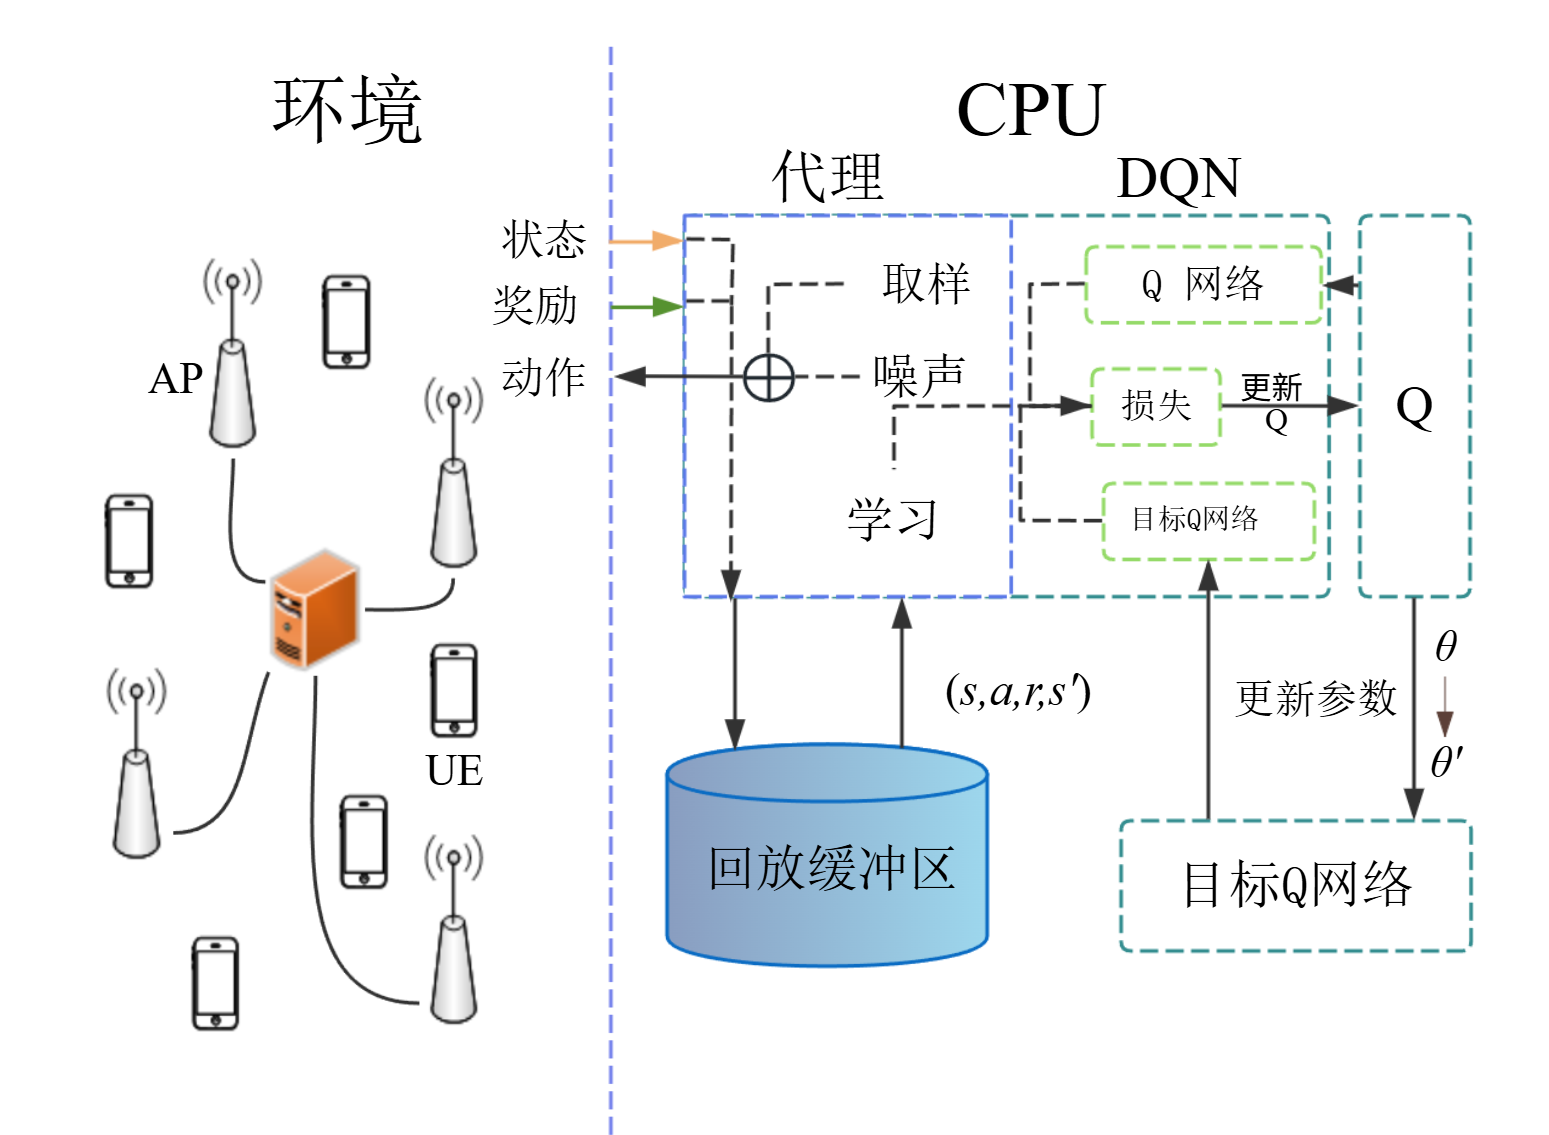
\includegraphics[width=3.5in] {fig3}
\caption{Network architecture of MADQIN.}
\label{fig3}
\end{figure}

\renewcommand{\thefootnote}{\ding{\numexpr192+\value{footnote}}}
\begin{algorithm}[t]
    \renewcommand{\algorithmicrequire}{\textbf{Input:}}
    \renewcommand{\algorithmicensure}{\textbf{Output:}}
    \caption{MADQIN Algorithm}
    \label{DQN}
    \begin{algorithmic}[1]
        \State $\emph{Input:}$ Episode times $N_e$, exploration times $T$, target network update frequency $T_u$, discount factor $\gamma$, learning rate $\alpha$, and random data quantity $R_q$. % input
      	  \State $\emph{Initialization:}$ Initialize MADQIN $Q(s,a;\omega _q)$ parameter $\omega _q$ with He initialization method.
    			% for loop
        \For {$k=1$ to $N_e$}
        		\State Creating environment object $  \mathcal{O} _e$ and neural network object $  \mathcal{O} _d$.
        		\State Initialize status $s^1$.
        		% for loop
	        \For {$ \jmath  =1$ to $T$}
	            % if ... else
		        \If {$ \jmath  < R_q$}
		            \State Randomly select action set $a^t\in \mathcal{A}$ with uniform probablity. 
		        \Else
		            \State Select action $a^t$ by \eqref{eqn-39}.
		        \EndIf
		        \State Execute action $a^t$, obtain reward $r^t$, and next state $s^{t+1}$.
		        \State Store the transaction$(s^{t},a^{t},r^{t},s^{t+1})$.
		        \State Minimizing the loss to update the MADQIN network.
		        \State \begin{align} L^t(\omega _q^t)&= (r_{s,a}^t+\gamma \underset{a^{t+1}}{\text{max}}Q(s^{t+1},a^{t+1};\omega_{target})
		        					\nonumber\\&\quad-Q(s^t,a^t;\omega_q ^t) )^2. \nonumber\end{align}
	        \EndFor
        \EndFor
        \State $\emph{Output:}$ Learned DQN $Q(s,a;\omega _q)$. % output
        
		\end{algorithmic}
\end{algorithm}

\section{MADQIN算法设计}

考虑到模数转换器（ADC）分辨率的离散特性，本章采用离散动作空间的深度Q网络（DQN）作为优化框架，并设计了一种离散动作空间的多智能体深度Q集成网络（MADQIN）。如图 \ref{fig3} 所示，该算法架构主要由Q网络（Q-Network）和目标Q网络（Q-target）两个神经网络构成。MADQIN通过Q网络预测系统内智能体动作的最大Q值，并将其作为预测奖励 $r_p$；随后智能体选择Q值最高的动作执行，以获取实际奖励 $r$。此外，目标Q网络用于预测下一状态的Q值 $r_t$，并将 $r$ 与 $r_t$ 之和作为真实奖励 $r'$。通过迭代不断更新Q网络的参数 $\omega_q$，以最小化 $r_p$ 与 $r'$ 之间的误差。该优化目标的具体表达式为
\begin{equation}\omega  _q^* = \underset{\omega  _q}{\text{argmin}} \frac{1}{2} (Q(s ,a ;\mathbf{\omega  } _q)-r_s^a)^2.\end{equation}
$\omega_q$ 的梯度计算方法为：
\begin{equation}\nabla \omega _q = (Q(s,a;\omega _q)-r_s^a)\nabla _{\omega _q}Q(s,a;\omega _q).\end{equation}

在深度强化学习（DRL）环境中，本文将MADQIN的输出层维度定义为 $[M, AD]$，其中 $AD$ 表示每个接入点（AP）可采用的ADC分辨率可选数量。该网络的输出旨在预测 $M$ 个AP在给定状态集合下执行每一种可能动作对应的Q值。为选取最优动作策略，本文求解使Q值最大化的动作 $a^*$。该策略通过融合 $M$ 个深度Q网络（DQN）的预测结果实现，确保在多AP环境下选中最优的ADC分辨率配置。最优动作集合可通过如下公式求得，
\begin{equation}\label{eqn-39}a^* = \underset{a}{\text{argmax}}Q(s,a;\omega  _q).\end{equation}

MADQIN网络的输入与输出设计与DMAGNN-AC的组件设计保持一致。不同于传统方法中通过贪心策略最大化样本多样性的思路，本文选择在初始 $\jmath$ 步采用随机动作策略，并将这些动作产生的数据纳入经验回放缓冲区。该方式提升了模型的鲁棒性与适应性。通过一系列实验验证，本文证明该随机动作策略在研究的特定场景下表现出更优效果。此外，为进一步提升算法性能，本文在执行动作时引入高斯随机噪声，其表达式为
\begin{equation}a := \left [ a^*+\mathbf{n} \right   ]^{b_m^\text{max}}_{b_m^\text{min}} .\end{equation}

\begin{table}[t]
  \begin{center}\label{table1}
    \caption{System basic parameter settings.}
    \begin{tabular}{@{}lll@{}}
			\toprule
                          & \textbf{Parameters}                        & \textbf{Values} \\ \midrule
 							    				 & Carrier frequency                   	& 1.9 GHz             \\
                          & Bandwidth                    				 	& 20 MHz          \\
                          & Noise figure           & 9 dB   \\
                          & AP antenna height & 15 m     \\
                          & User antenna height   & 1.65 m           \\
                          & Coherence interval length $\tau$        & 200\\
                          & Pilot length $\tau_\text{p}$   & 20  \\
                          & Pilot transmission power $\rho_\text{p}$              & 200 mW             \\
                          & ADC resolution $b_m$            &10   \\
                          & $M$, $K$, $N$    & 100, 20, 4\\
                          &$\delta _\text{sh}$, $L$, $d_1$, $d_0$   & 8 dB, 140.7 dB, 50 m, 10 m     \\\midrule
			\end{tabular}
  \end{center}
\end{table}

\begin{table}[t]
  \begin{center}\label{table2}
    \caption{Neural Network Parameter Settings.}
    \begin{tabular}{@{}lll@{}}
			\toprule
			                          & \textbf{Parameters}                        & \textbf{Values} \\ \midrule
			\multirow{6}{*}{DMAGNN-AC} & Discount factor $\gamma$                   & 0.1             \\
			                          & Learning rate $\alpha $                    & 0.001           \\
			                          & Size of experience replay buffer $\mathcal{B}$           & 10000   \\
			                          & Frequency of updating initial trial status $\mathcal{H}$ & 500     \\
			                          & Update neural network parameter weights $\tau$   & 0.005           \\
			                          & Warm up times   $\mathcal{W}$              & 256             \\ \midrule
			\multirow{5}{*}{MADQIN}   & Learning rate   $\alpha $                  & 0.001           \\
			                          & Discount factor $\gamma$                   & 0.1             \\
			                          & Size of experience replay buffer  $\mathcal{B}$         & 1000     \\
			                          & Batch size      $\varsigma$                & 200             \\
			                          & Warm up times  $\mathcal{W}$               & 200             \\ \midrule
			\end{tabular}
  \end{center}
\end{table}
MADQIN的详细执行流程总结于本页顶部的算法 \ref{DQN} 中。

\section{数值结果与分析}
在本节中，本文通过一系列实验结果，对搭载非线性功率放大器（PA）与低分辨率模数转换器（ADC）的CF‑mMIMO系统性能进行阐述与分析。如无特殊说明，均采用表Ⅰ所示的标准实验参数配置。

本文在研究中沿用文献 \cite{paper15} 中非线性PA模型的系数设置，其中 $a_1=13.85$，$a_3=-4.074$。对于大尺度衰落系数模型 $\beta_{mk}$，本文采用特定建模方式，以精准反映实际通信环境中的信号衰减特性。

\begin{equation}\beta _{mk} = \text{PL}_{mk}\cdot 10^{\frac{\delta _{\text{sh}^zmk}}{10} },\end{equation}
其中 $10^{\frac{\delta_{\text{sh}^zmk}}{10}}$ 用于模拟阴影效应，$z_{mk}\sim \mathcal{CN}(0,1)$。变量 $\text{PL}_{mk}$ 表示路径损耗，遵循文献 \cite{paperI4} 提出的三斜率模型。路径损耗（单位：dB）为
\begin{equation}\text{PL}_{m k}=\left\{\begin{array}{l}
-L-35 \log _{10}\left(d_{m k}\right), \text { if } d_1<d_{mk} \\
-L-15 \log _{10}\left(d_{1}\right)-20 \log _{10}\left(d_{m k}\right), \\
\quad\quad\quad\quad\quad\quad\quad\quad\quad\quad\quad\text { if } d_{0}<d_{m k} \leq d_{1} \\
-L-15 \log _{10}\left(d_{1}\right)-20 \log _{10}\left(d_{0}\right), \text { if } d_{m k} \leq d_{0}
\end{array}\right.\end{equation}

需要注意的是，当 $d_{mk}<d_{1}$ 时不存在阴影效应。

为验证所提算法的性能，本文将其与基础的全功率发射方法进行对比。大量实验结果表明，在每种环境下约 2000 步即可达到理想效果。两种算法的相关参数总结于表Ⅱ中。

\begin{figure}
\centering
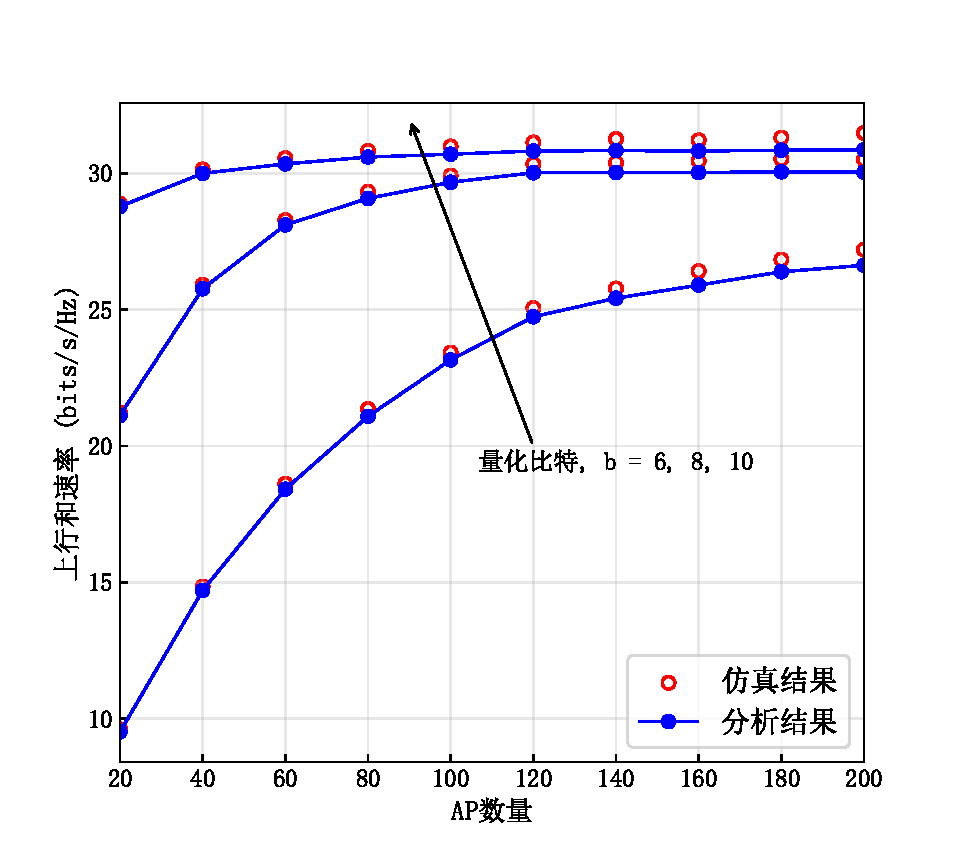
\includegraphics[width=3.2in] {MonteCarlo}
\caption{Achievable uplink sum-rate versus the number of APs, with $K=20$, $N=20$.}
\label{MonteCarlo}
\end{figure}

首先，图 \ref{MonteCarlo} 给出了上行可达和速率与接入点（AP）数量之间的关系。此外，本文对式 \eqref{eqn-23} 对应的“解析结果”与式 \eqref{eqn-22} 给出的“仿真结果”进行了对比分析。“仿真结果”通过蒙特卡洛方法，在 $10^4$ 次独立同分布（i.i.d.）信道实现下完成验证。可以清晰地看出，“仿真结果”与“解析结果”高度吻合，充分证明了推导结果的准确性，为后续相关理论研究奠定了坚实基础。

\begin{figure}
\centering
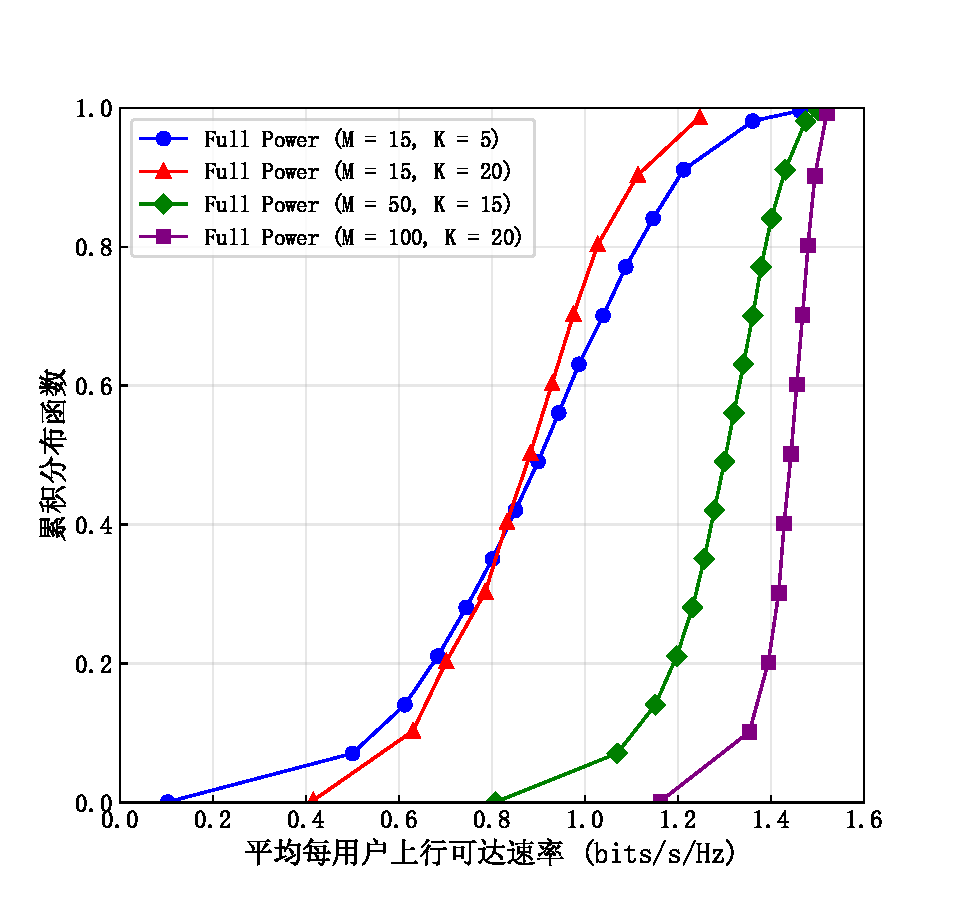
\includegraphics[width=3.2in] {fig4}
\caption{Uplink per-user rate under different numbers of APs and UEs during full power transmission, with $N$ = 4, $b_m$ = 10.}
\label{fig4}
\end{figure}


图 \ref{fig4} 给出了全功率传输时，不同接入点（AP）与用户设备（UE）数量下单用户速率的累积分布函数（CDF）曲线。可以看出，当 $M=15$ 时，随着UE数量增加，平均单用户速率呈下降趋势。这是因为随着UE密度升高，导频污染与多用户干扰愈发严重。值得注意的是，尽管平均速率有所下降，用户速率下界却有所提升。主要原因是：当AP数量远大于UE数量时，系统尚未达到最大服务容量。而当UE数量超过AP数量时，用户速率会受到明显干扰，这一问题可通过增加AP数量来缓解。随着UE与AP数量增加，CDF曲线逐渐右移，并最终收敛于共同上限值 $1.5$ bits/s/Hz。结果表明：在本文研究场景中，单纯增加AP与UE数量并不能无限制提升用户速率，但可以提高用户速率下界，增强系统数据传输的稳定性。
这体现了CF‑mMIMO系统的特点：能够为所有用户提供稳定、均匀的服务质量。

\begin{figure}
\centering
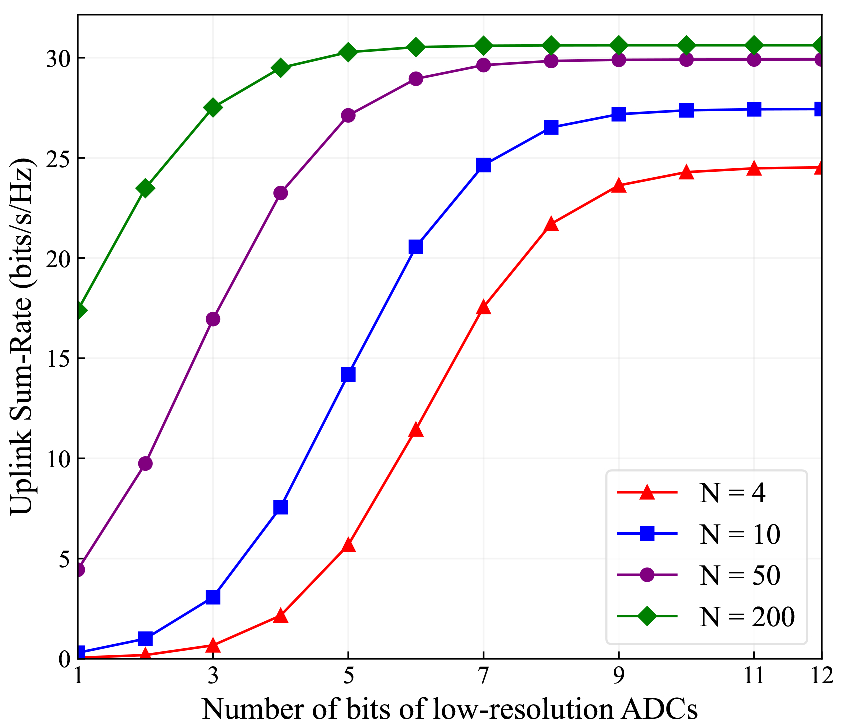
\includegraphics[width=3.2in] {fig5}
\caption{The relationship between uplink sum-rate and the number of bits of low resolution ADCs under different numbers of AP antennas, with $M$ = 100, $K$ = 20.}
\label{fig5}
\end{figure}
\begin{figure}
\centering
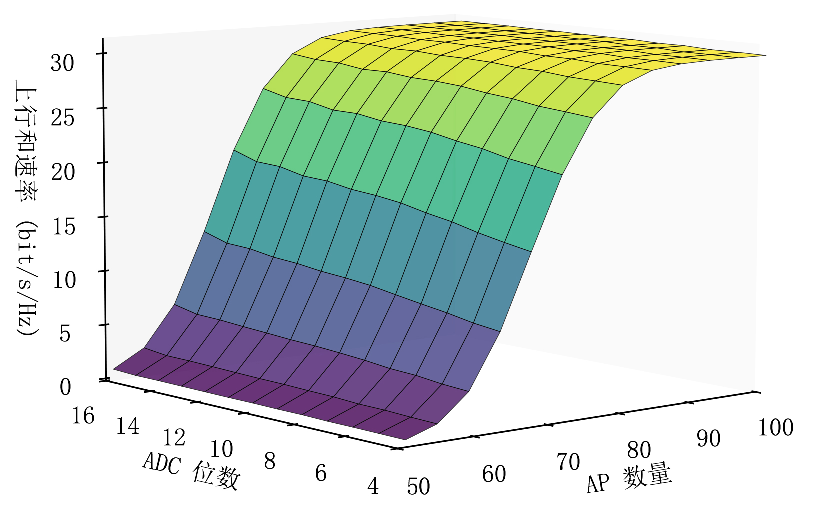
\includegraphics[width=3.5in] {fig6}
\caption{The impact of ADC bit count and AP count on uplink sum-rate, with $K$ = 20.}
\label{fig6}
\end{figure}

图 \ref{fig5} 和图 \ref{fig6} 分别展示了在多种影响因素存在时，低分辨率ADC的比特位数对上行用户和速率的影响。在每组实验中，假设所有AP配备相同分辨率的ADC。
从两幅图中均可明显看出：在达到峰值速率之前，提高ADC分辨率能够显著提升用户速率。但在更大尺度下，AP数量成为决定用户速率的主要因素，这表明增加AP数量可以补偿由低分辨率ADC带来的速率损失。此外，天线数量不足会导致系统无法达到用户速率的最大潜在性能。如图 \ref{fig5} 所示，仅当 $N \ge 50$ 时用户速率才接近极限，这说明在实际部署中，需根据AP数量合理配置天线数量，才能充分发挥系统性能。同时，随着天线数量增加，单用户速率逐渐趋于上限 $1.5$ bits/s/Hz，与前文结论一致。当 $N$ 相对于
${\rho _\text{u}}\sum\limits_{m = 1}^M {\alpha _m}(1 - {\alpha _m})\left( \sum\limits_{k = 1}^K {\beta _{mk}}\Omega _k + 1 \right){\gamma _{mk}}$
足够大时，其对用户速率的影响逐渐减弱。此外，图 \ref{fig5} 与图 \ref{fig6} 中的峰值速率基本一致，表明单纯提升ADC分辨率与AP天线数量无法突破系统固有的速率上限。

\begin{figure}
\centering
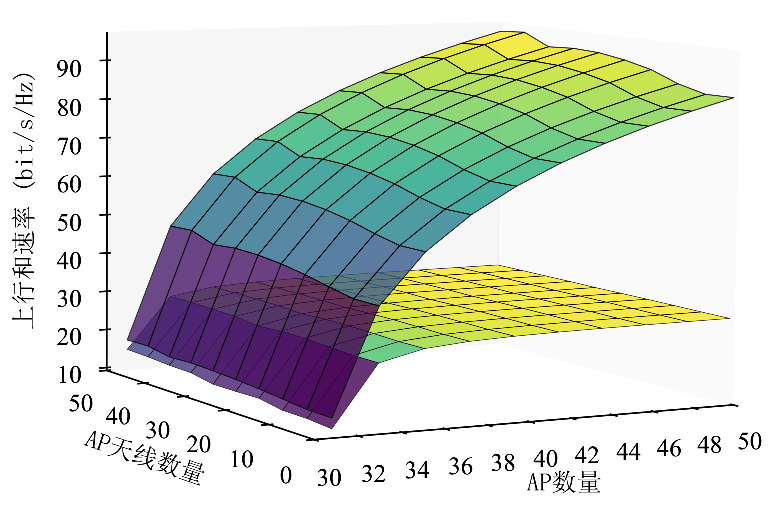
\includegraphics[width=3.5in] {fig7}
\caption{Comparing the uplink sum-rate in a CF-mMIMO system with nonlinear PAs and low-resolution ADCs versus the ideal hardware scenario, with $b_m$ = 10.}
\label{fig7}
\end{figure}

随后，本文对比分析了理想硬件条件与非理想硬件条件下，CF‑mMIMO系统在不同AP数量与AP天线数量时的可达用户速率。如图 \ref{fig7} 所示，在理想硬件条件下，随着AP数量与天线数量的增加，用户和速率最高可超过 90 bits/s/Hz。然而，受非线性PA**与低分辨率ADC的影响，用户和速率的峰值被限制在 30 bits/s/Hz 左右。结果表明，硬件损伤的存在使系统速率下降近 70\%，这凸显了对含硬件损伤系统开展深入研究的必要性。
\begin{figure}
\centering
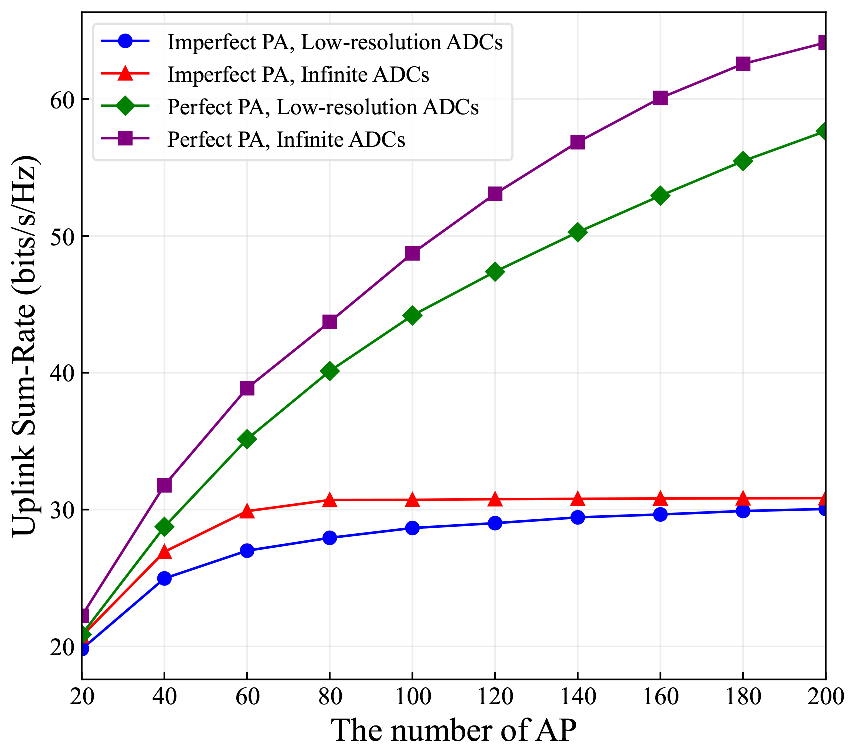
\includegraphics[width=3.2in] {compare}
\caption{Rate comparison based on different hardware impairments, with $b_m$ = 10, $K$ = 20.}
\label{compare}
\end{figure}

随后，为深入分析导致用户速率显著下降的主要因素，图 \ref{compare} 通过控制硬件损伤变量设计了对比实验。实验结果表明，在假设ADC具有无限分辨率的理想条件下，PA的非线性成为限制用户速率上限的关键因素，这有力支撑了我们对式 \eqref{eqn-23} 的分析结论。

\begin{figure}
\centering
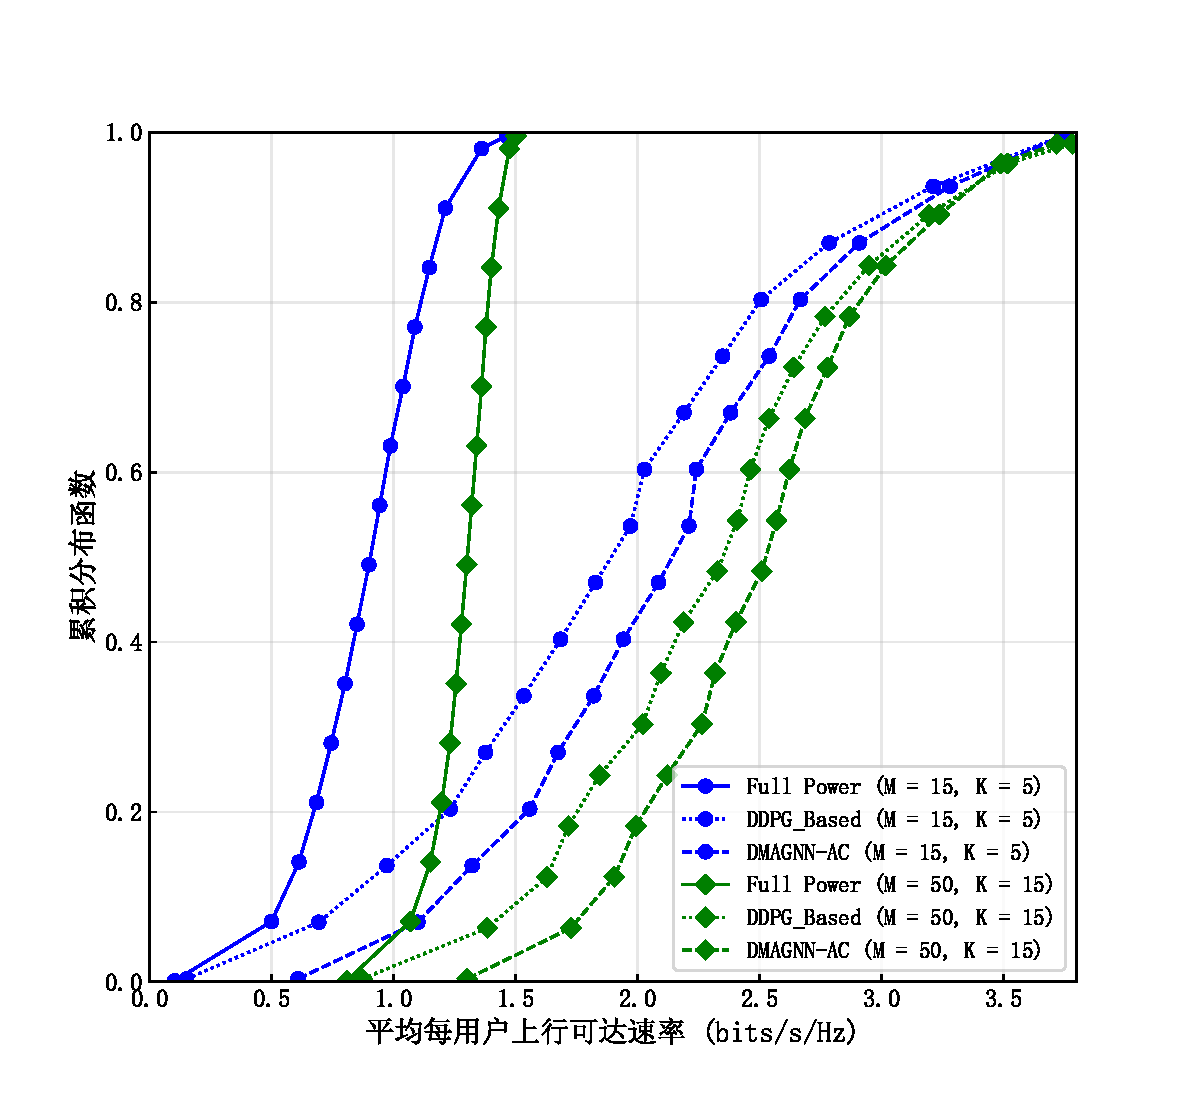
\includegraphics[width=3.2in] {fig10}
\caption{Comparison of per-user rate between full power transmission, DDPG$\_$Based, and DMAGNN-AC algorithm, with $b_m$ = 10, $N$ = 4.}
\label{fig10}
\end{figure}
\begin{figure}
\centering
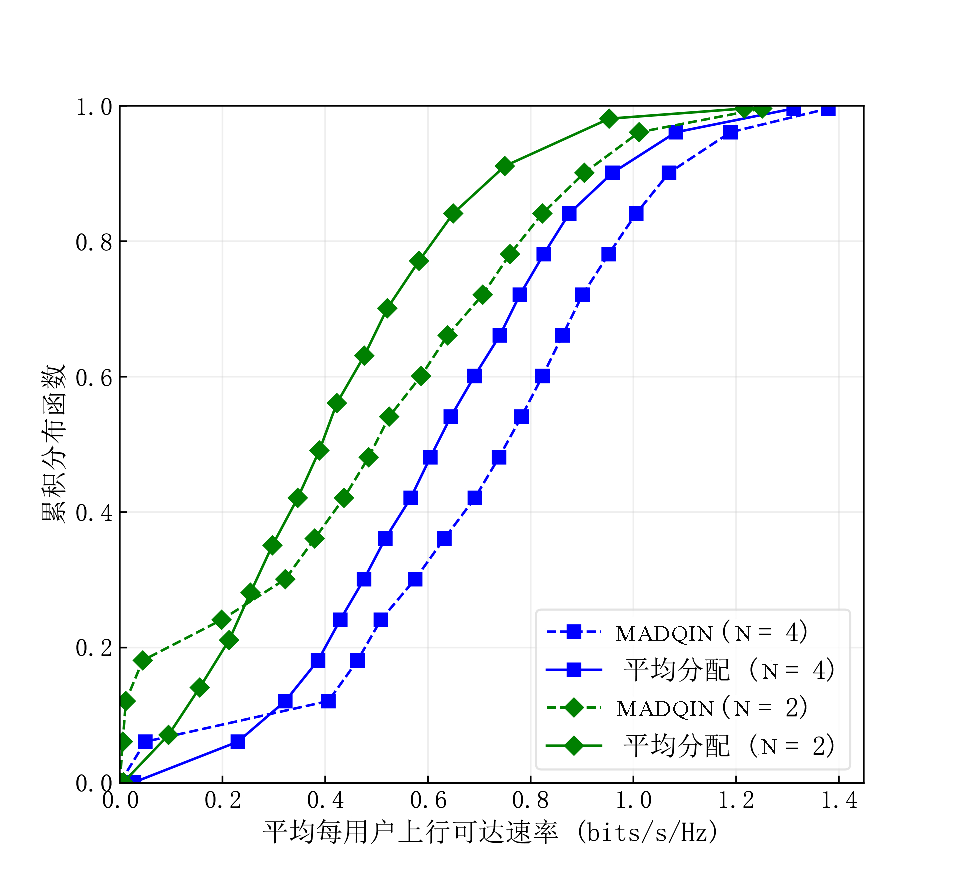
\includegraphics[width=3.2in] {fig11}
\caption{Comparison of average allocation and the MADQIN algorithm under the same total bit count, with $b_\text{total}$ =135, $M$ = 15, and $K$ = 5.}
\label{fig11}
\end{figure}

接下来，本文利用所提算法对整个系统中各AP与UE的实验参数进行精细调控，从不同角度验证算法带来的性能提升。图 \ref{fig10} 对比了DMAGNN‑AC算法与全功率传输策略、DDPG算法的优化性能。DDPG算法通过与环境交互探索逐步逼近最优解，在达到全功率策略性能上限后，可将单用户速率进一步提升 $2.8$ bit/s/Hz。此外，在引入DMAGNN作为特征提取模块后，速率的累积分布曲线相对DDPG进一步右移，验证了DMAGNN通过干扰建模与多尺度特征融合，能够提升算法收敛性能并改善最小用户速率。不同AP‑UE配置下的对比结果表明，系统最高用户速率稳定在 $3.8$ bit/s/Hz 左右，即为用户速率的最终性能边界。

如图 \ref{fig11} 所示，在总比特数保持恒定的前提下，本文所提的MADQIN算法相比平均分配策略在性能上有显著提升。随着天线数量增加，用户速率呈逐步上升趋势。值得注意的是，调整AP的ADC分辨率仅能带来较小的性能增益。这一现象可由式 \eqref{eqn-23} 解释：速率主要由ADC总分辨率决定，无论信号是期望信号还是用户间干扰，仅有ADC量化噪声项与分辨率的具体分配有关。因此，该影响处于可接受范围内。

\begin{figure}
\centering
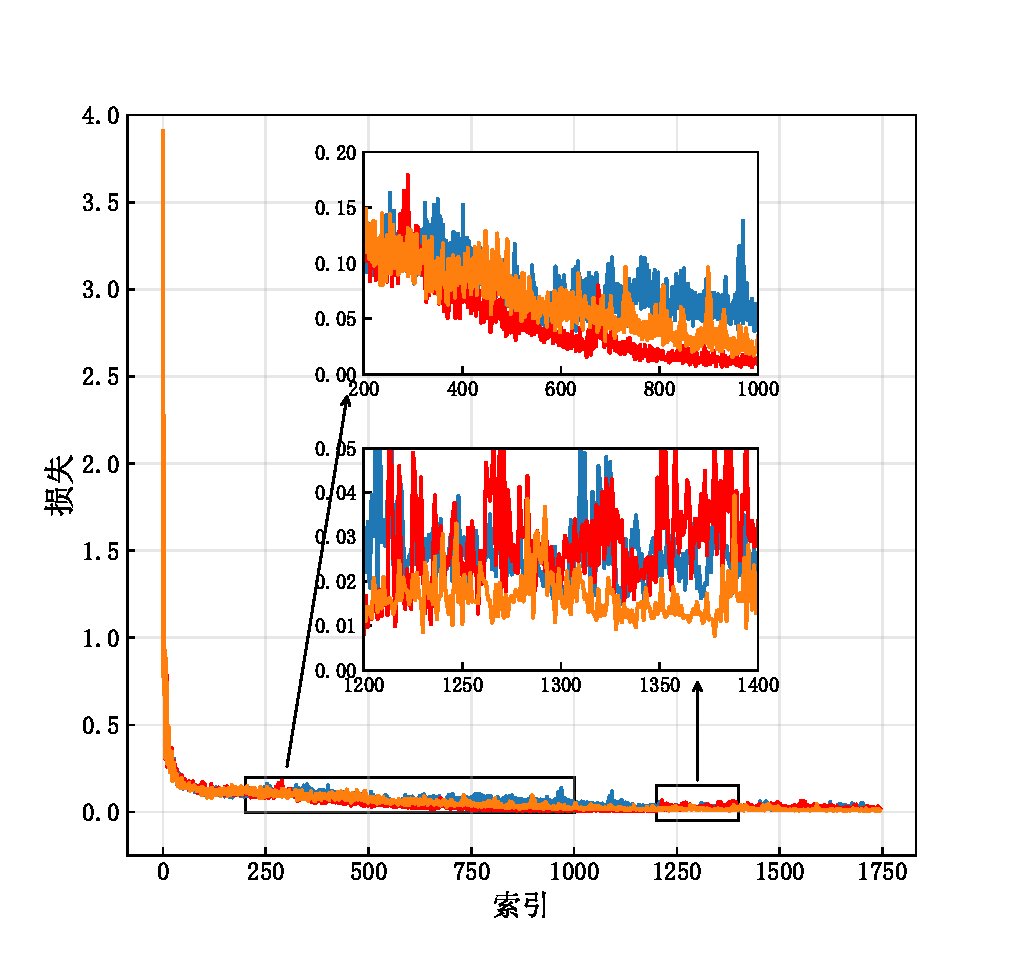
\includegraphics[width=3.2in] {fig8}
\caption{Convergence of DMAGNN-AC algorithm.}
\label{fig8}
\end{figure}
\begin{figure}
\centering
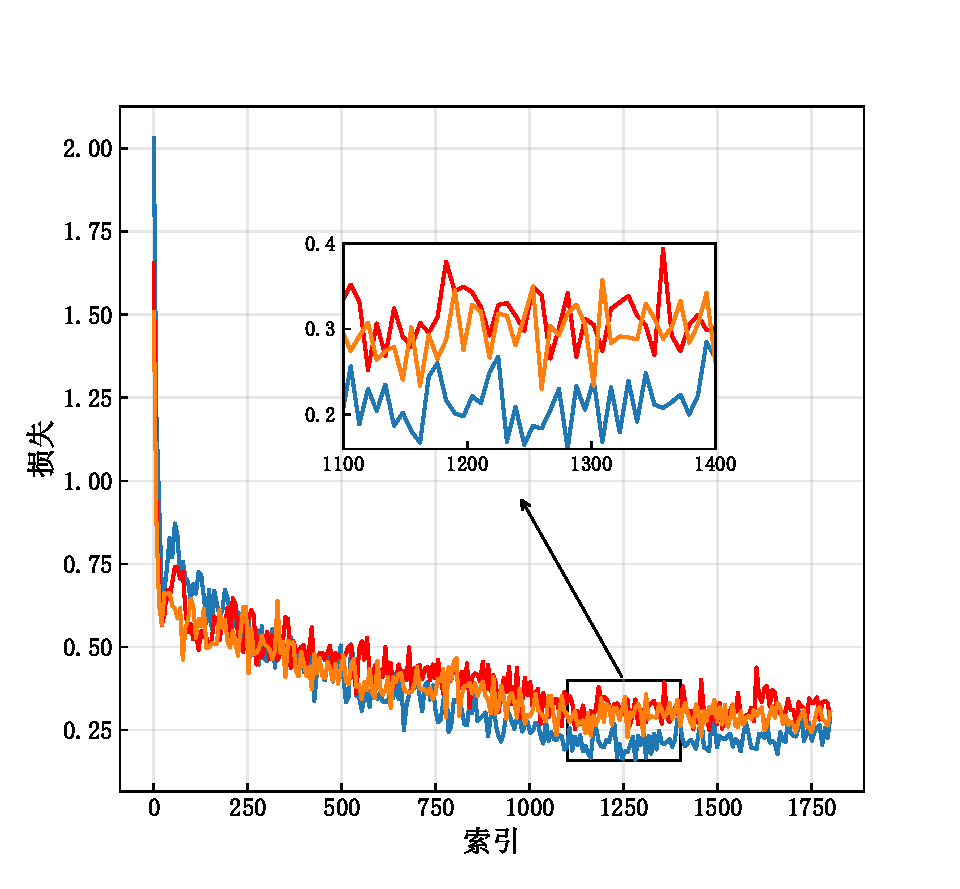
\includegraphics[width=3.2in] {fig9}
\caption{Convergence of MADQIN algorithm.}
\label{fig9}
\end{figure}

图 \ref{fig8} 和图 \ref{fig9} 分别给出了两种算法在迭代过程中的损失函数值。为使结果更具普适性，本文对三组损失结果进行了对比。可以看出，两种算法在迭代1200轮后均呈现出明显的收敛趋势，充分证明了两种算法均具备优异的性能稳定性。

\section{本章小结}
本文研究了存在非线性功率放大器（PA）与低分辨率模数转换器（ADC）场景下，CF‑mMIMO系统的上行数据传输问题，并推导出了可达用户速率的闭合表达式。研究结果表明，硬件性能会对系统性能产生显著影响。为补偿由非线性PA与低分辨率ADC造成的速率损失，本文提出一种基于深度强化学习的DMAGNN‑AC功率控制算法，以抑制来自其他用户的干扰。与全功率传输策略和DDPG算法相比，该算法可显著提升系统性能与最小用户速率下界。随后，本文利用MADQIN算法对ADC分辨率进行合理调整，使用户速率得到小幅提升。最后，通过深度强化学习算法验证了在CF‑mMIMO系统中使用低质量硬件的可行性。

\chapter{非理想硬件条件下去蜂窝大规模MIMO系统的URLLC服务资源分配策略}\label{chap:MIMOLP}

在第三章中，本文研究了块长足够长条件下非理想硬件CF-mMIMO系统的可达速率优化问题。然而，工业自动化等物联网关键应用对URLLC提出了毫秒级时延与极高可靠性的严苛需求，短传输块特性使得第三章的长码块假设不再适用。为此，本章聚焦硬件损伤条件下CF-mMIMO系统的URLLC性能优化问题，构建了非线性PA的损伤模型，推导了有限块长下上行链路UE速率闭合表达式。为降低传统优化算法的计算复杂度，提出基于GNN与DRL融合的智能功率控制策略，通过图嵌入技术建模UE空间相关性，动态抑制硬件损伤与时变信道干扰。所提方案在保持毫秒级时延的同时，为工业自动化等物联网应用提供理论与技术支撑。

\section{引言}

随着移动通信技术的不断演进，第五代及未来移动通信网络正推动智能制造、智能交通等物联网应用的快速发展。该网络主要承载超可靠低延迟通信（URLLC）、增强型移动宽带（eMBB）和大规模机器类通信（mMTC）三大核心场景，各场景对可靠性、时延、传输速率及连接密度的服务质量提出了差异化且严苛的要求。其中，URLLC以极端事件响应为目标，要求时延控制在1-10毫秒、误块率低至$10^{-5}$-$10^{-7}$，成为支撑机器人协同控制、自动驾驶等关键任务的核心技术。然而，URLLC的短传输块特性使得传统香农容量理论难以直接适用，现有蜂窝网络架构在保障服务质量方面也面临结构性瓶颈。

去蜂窝大规模多输入多输出（CF-mMIMO）系统作为新一代网络架构，为URLLC服务提供了创新性解决方案。该系统通过分布式部署大量接入点（AP），并与中央处理单元（CPU）协同工作，有效消除蜂窝边缘干扰，实现全域均匀服务覆盖。与传统集中式大规模MIMO相比，CF-mMIMO缩短了AP与UE的空间距离，显著降低信号传播衰落；其稀疏空间布局与多元宏观特征能够稳定信道状态，形成独特的信道硬化效应。这些技术特性为URLLC可靠性提升提供了坚实保障，展现出显著的技术优势。

本章以CF-mMIMO系统的URLLC服务为研究对象，重点探讨硬件损伤条件下的功率分配优化问题。与第三章同时考虑PA非线性与低分辨率ADC的联合影响不同，本章聚焦于UE端非线性PA这一核心硬件损伤因素，通过简化AP端为理想高精度ADC，深入剖析PA非线性对URLLC短包传输性能的内在影响机理。在此基础上，采用无记忆多项式模型刻画PA失真特性，推导有限块长下上行链路用户速率的解析表达式，为后续智能功率控制策略的设计奠定理论基础。

\section{模型设计}

本章在第三章系统模型的基础上进行简化，重点研究仅存在PA非线性硬件损伤的场景。相较于第三章同时考虑PA非线性和低分辨率ADC的复杂模型，本章假设AP端配备理想的高精度ADC（即$b_m \to \infty$，$\alpha_m = 1$），从而能够更加聚焦地分析PA非线性对URLLC服务性能的影响。该简化模型不仅有助于理论推导的清晰性，更能深入揭示硬件损伤与URLLC性能之间的内在关联机制。

\subsection{信道估计}

考虑一个上行链路CF-mMIMO系统，该系统由$M$个配备$N$根天线的AP和$K$个单天线UE构成。第$m$个AP与第$k$个UE之间的信道向量可建模为
\begin{equation}
\mathbf{g}_{mk} = \beta_{mk}^{1/2} \mathbf{h}_{mk},
\end{equation}
其中，$\beta_{mk}$表示大尺度衰落效应，$\mathbf{h}_{mk}$为小尺度衰落向量，其各元素服从独立同分布的复高斯分布$\mathcal{CN}(0,1)$。

为刻画UE端PA的非线性特性，采用无记忆多项式模型进行建模。经非线性PA处理后，第$k$个UE发送的导频信号可表示为
\begin{equation}
\boldsymbol{\phi}_k = \tilde{a}_1\boldsymbol{\varphi}_k + \tilde{a}_3\boldsymbol{\varphi}_k\|\boldsymbol{\varphi}_k\|^2,
\end{equation}
其中，$\tilde{a}_1 = a_1\sqrt{\tau_\text{p}}$，$\tilde{a}_3 = a_3\tau_\text{p}\sqrt{\tau_\text{p}}$，$a_1$和$a_3$分别为无记忆多项式模型的一阶和三阶复系数。

第$m$个AP接收到的导频信号为
\begin{equation}
\mathbf{Y}_{\text{p},m} = \sqrt{\rho_\text{p}}\sum_{k=1}^{K}\mathbf{g}_{mk}\boldsymbol{\phi}_k^H + \mathbf{W}_{\text{p},m},
\end{equation}
其中，$\rho_\text{p}$为导频信号功率，$\mathbf{W}_{\text{p},m}$为加性高斯白噪声矩阵。

鉴于本章假设AP配备理想高精度ADC，即$\alpha_m = 1$且量化噪声可忽略不计，AP可直接对接收信号进行投影处理。将接收信号$\mathbf{Y}_{\text{p},m}$投影至导频序列$\boldsymbol{\varphi}_k$，得到
\begin{equation}
\check{\mathbf{y}}_{\text{p},mk} = \sqrt{\rho_\text{p}}\sum_{k'\in\mathcal{P}_k}(\tilde{a}_1+\tilde{a}_3\tau_\text{p})\mathbf{g}_{mk'} + \mathbf{W}_{\text{p},m}\boldsymbol{\varphi}_k,
\end{equation}
其中，$\mathcal{P}_k$表示与第$k$个UE共享相同导频序列的UE集合。

采用最小均方误差（MMSE）估计算法，信道向量$\mathbf{g}_{mk}$的估计值可表示为
\begin{equation}
\hat{\mathbf{g}}_{mk} = c_{mk}\check{\mathbf{y}}_{\text{p},mk},
\end{equation}
其中，MMSE估计系数$c_{mk}$由下式给出：
\begin{equation}
c_{mk} = \frac{\sqrt{\tau_\text{p}\rho_\text{p}}\beta_{mk}(a_1+a_3\tau_\text{p})}{\tau_\text{p}\rho_\text{p}\sum_{k'\in\mathcal{P}_k}(a_1+a_3\tau_\text{p})^2\beta_{mk'}+1}.
\end{equation}

信道估计向量第$n$个分量的均方值可推导为
\begin{equation}
\gamma_{mk} = \frac{\tau_\text{p}\rho_\text{p}\beta_{mk}^2(a_1+a_3\tau_\text{p})^2}{\tau_\text{p}\rho_\text{p}\sum_{k'\in\mathcal{P}_k}(a_1+a_3\tau_\text{p})^2\beta_{mk'}+1}.
\end{equation}

定义信道估计误差向量为$\tilde{\mathbf{g}}_{mk} = \mathbf{g}_{mk} - \hat{\mathbf{g}}_{mk}$，其各元素服从复高斯分布$\mathcal{CN}(0, \beta_{mk}-\gamma_{mk})$，反映了信道估计的不确定性。

\subsection{上行数据传输}

在上行数据传输阶段，考虑UE端PA的非线性特性。第$k$个UE经非线性PA处理后的输出信号可表示为
\begin{equation}
y_k = \sqrt{\rho_\text{u}}\left(\tilde{a}_{1k}q_k + \tilde{a}_{3k}q_k|q_k|^2\right),
\end{equation}
其中，$\tilde{a}_{1k} = a_1\sqrt{\eta_k}$，$\tilde{a}_{3k} = a_3\eta_k\sqrt{\eta_k}$，$\eta_k$为功率控制系数，需满足功率约束条件$|a_1|^2\eta_k + 2(a_1^*a_3+a_1a_3^*)\eta_k^2 + 6|a_3|^2\eta_k^3 \leq 1$。

第$m$个AP接收到的上行信号为
\begin{equation}
\mathbf{y}_{\text{u},m} = \sqrt{\rho_\text{u}}\sum_{k=1}^{K}\left(\tilde{a}_{1k}\mathbf{g}_{mk}q_k + \tilde{a}_{3k}\mathbf{g}_{mk}q_k|q_k|^2\right) + \mathbf{w}_{\text{u},m},
\end{equation}
其中，$\rho_\text{u}$为上行数据传输功率，$\mathbf{w}_{\text{u},m} \sim \mathcal{CN}(\mathbf{0},\mathbf{I}_N)$为加性高斯白噪声。

在CPU处，采用MF接收信号进行处理，第$k$个用户的合并信号为
\begin{equation}
r_{\text{u},k} = \sum_{m=1}^{M}\hat{\mathbf{g}}_{mk}^H\mathbf{y}_{\text{u},m}.
\end{equation}

\subsection{可达速率分析}

为分析系统性能，将接收信号$r_{\text{u},k}$分解为多个分量：
\begin{equation}
r_{\text{u},k} = \text{ES}_k \cdot q_k + \text{BU}_k \cdot q_k + \sum_{k'\neq k}^{K}\text{I}_{kk'} \cdot q_{k'} + \sum_{k'\neq k}^{K}\text{NB}_{kk'} \cdot q_{k'} + \text{N}_k,
\end{equation}
其中，各分量分别表示期望信号（ES）、波束成形增益不确定性（BU）、用户间干扰（I）、非线性干扰（NB）以及加性噪声（N）。

基于信道估计误差模型$\mathbf{g}_{mk} = \hat{\mathbf{g}}_{mk} + \tilde{\mathbf{g}}_{mk}$及MMSE估计的统计特性，期望信号分量可推导为
\begin{equation}
\text{ES}_k = N\sqrt{\rho_\text{u}}(\tilde{a}_{1k}+\tilde{a}_{3k})\sum_{m=1}^{M}\gamma_{mk}.
\end{equation}

加性噪声分量的方差为
\begin{equation}
\mathbb{E}\{|\text{N}_k|^2\} = N\sum_{m=1}^{M}\gamma_{mk}.
\end{equation}

假设总干扰$\Theta_k$包含波束成形增益不确定性、UE间干扰和PA非线性损伤三个主要部分。其方差可简化为如下表达式：
\begin{equation}
\mathbb{E}\{|\Theta_k|^2\} = N\rho_\text{u}\sum_{k'=1}^{K}\Omega_{k'}\sum_{m=1}^{M}\gamma_{mk}\beta_{mk'} + 3N\rho_\text{u}|a_3|^2\eta_k^3\left(\sum_{m=1}^{M}\gamma_{mk}\right)^2,
\end{equation}
其中，$\Omega_k = |a_1|^2\eta_k + 2(a_1^*a_3+a_1a_3^*)\eta_k^2 + 6|a_3|^2\eta_k^3$表征第$k$个UE的有效发射功率。

\subsection{上行可达速率闭合表达式}

基于前述分析结果，第$k$个UE的上行可达速率可表示为
\begin{equation}
R_{\text{u},k} = \log_2\left(1 + \text{SINR}_k\right),
\end{equation}
其中，$\text{SINR}_k$的闭合表达式为
\begin{equation}\label{SINR}
\text{SINR}_k = \frac{N\rho_\text{u}|\tilde{a}_{1k}+\tilde{a}_{3k}|^2\left(\sum_{m=1}^{M}\gamma_{mk}\right)^2}{\rho_\text{u}\sum_{k'=1}^{K}\Omega_{k'}\sum_{m=1}^{M}\gamma_{mk}\beta_{mk'} + 3\rho_\text{u}|a_3|^2\eta_k^3\left(\sum_{m=1}^{M}\gamma_{mk}\right)^2 + \sum_{m=1}^{M}\gamma_{mk}}.
\end{equation}

上述闭合表达式从理论上刻画了PA非线性对系统性能的内在影响机制。具体而言，分子项$|\tilde{a}_{1k}+\tilde{a}_{3k}|^2$量化了PA非线性导致的期望信号功率衰减程度；分母中的$3\rho_\text{u}|a_3|^2\eta_k^3(\sum_{m}\gamma_{mk})^2$项则表征了PA非线性引入的自干扰分量对有效信干噪比的劣化作用。值得注意的是，当$a_3 = 0$时，即理想线性PA条件下，该表达式可退化为经典大规模MIMO系统的性能分析结果，验证了推导的正确性。

相较于第三章式(3-23)所给出的联合硬件损伤模型，本章表达式通过剔除ADC相关的量化噪声项$\Psi_k$及量化系数$\alpha_m$，聚焦于硬件损伤对URLLC场景的影响，更重要的是为后续URLLC性能分析与功率控制算法设计提供了更为聚焦的理论基础，便于深入揭示PA非线性在短包传输场景下的独特影响规律。

\section{可实现URLLC速率}
传统的香农容量是在假设码字长度趋于无穷大、解码错误概率趋近于零的理想条件下推导的。然而，在URLLC场景下，由于对时延和可靠性的极高要求，实际通信往往采用有限块长编码，此时香农容量理论已不再适用。为准确刻画有限块长下的系统性能，URLLC通常采用有限块长编码理论对可实现速率进行分析。

URLLC服务的核心性能评估指标主要涵盖可靠性与时延两个关键维度。可靠性指标采用误块率（Block Error Rate, BLER）$\varepsilon_k$进行量化，该参数表征传输数据包在解码过程中发生错误的概率。基于有限块长信息论的理论框架，第$k$个用户设备的误块率可近似表达为
\begin{equation}
\varepsilon_k \approx Q\left(\frac{nC_k - L_k}{\sqrt{nV_k}}\right),
\end{equation}
式中$n$表示传输块长参数，$L_k$为传输比特数量，$C_k = \log_2(1 + \text{SINR}_k)$为信道容量函数，$V_k = (\log_2 e)^2(1 - (1 + \text{SINR}_k)^{-2})$为信道色散参数。该数学表达式清晰揭示了误块率与信干噪比、传输块长之间的内在关联机制：当信道条件恶化或功率配置不足时，$\text{SINR}_k$的降低将导致信道容量$C_k$相应减小，从而引起误块率的升高。

依据3GPP TS 38.913技术标准规范，URLLC典型应用场景要求误块率不超过$10^{-5}$量级。本文假设所有用户设备采用统一的目标误块率设定值$\varepsilon_k = \varepsilon_{\text{th}} = 10^{-5}$，并基于此参数配置推导可实现速率的闭合表达式。

端到端传输时延$D_k$包含传输时延、处理时延以及排队时延等多个组成部分。本文研究重点聚焦于传输时延的分析，该时延分量由信道相干时间与系统带宽共同决定。具体而言，传输块长$n$满足以下关系式
\begin{equation}
n = \tau_{\text{c}} \cdot W,
\end{equation}
其中,$\tau_{\text{c}}$表示信道相干时间参数，$W$为系统带宽。根据3GPP标准规范，URLLC典型应用要求端到端时延不超过$1$毫秒，本文据此设定时延阈值$D_{\text{th}} = 1$ ms。

基于上述误块率模型与时延约束条件，根据有限块长信息论的理论基础\cite{polyanskiy2010channel}，第$k$个用户设备的URLLC可实现速率可近似表示为：
\begin{equation}
r_{\text{u},k} \approx C_k - \sqrt{\frac{V_k}{n}} Q^{-1}(\varepsilon_{\text{th}}),
\end{equation}
其中$Q^{-1}(\cdot)$为高斯$Q$函数的反函数。该近似表达式在传输块长$n \geq 100$信道使用条件下具有较高的计算精度，适用于URLLC短包传输场景的性能分析。

上述数学表达式系统揭示了URLLC可实现速率与误块率、时延约束之间的内在关联规律：一方面，目标误块率$\varepsilon_{\text{th}}$通过$Q^{-1}(\cdot)$函数直接影响速率修正项的大小，更严格的可靠性要求将导致更大的速率性能损失；另一方面，时延约束$D_{\text{th}}$通过决定传输块长$n$的取值，进而影响信道色散与速率修正幅度。需要特别指出的是，功率放大器非线性损伤会进一步劣化有效信干噪比性能，从而在有限块长传输条件下加剧速率损失效应。该表达式综合考虑了有限块长下的误码概率约束、时延约束以及非理想硬件损伤影响，更加贴合URLLC实际应用场景的技术要求，为后续资源分配算法设计与系统性能优化提供了坚实的理论基础。

\section{上行和速率最大化}
基于上述分析，本节建立非理想硬件条件下CF-mMIMO系统URLLC服务的功率控制优化问题。以最大化系统总可实现速率为目标，同时满足URLLC时延与可靠性约束，优化问题可表述为
\begin{align}
\max_{\boldsymbol{\eta}} \quad & \sum_{k=1}^{K} r_{\text{u},k}(\eta_k) \\
\text{s.t.} \quad & 0 \leq \eta_k \leq \eta_{\max}, \quad \forall k \in \mathcal{K}, \label{constraint:power} \\
& \varepsilon_k \leq \varepsilon_{\max}, \quad \forall k \in \mathcal{K}, \label{constraint:reliability} \\
& D_k \leq D_{\text{th}}, \quad \forall k \in \mathcal{K}, \label{constraint:delay}
\end{align}
其中，$\boldsymbol{\eta} = [\eta_1, \eta_2, \ldots, \eta_K]^T$表示功率控制向量，$r_{\text{u},k}(\eta_k)$的具体表达式由式(4-12)给出。约束条件\eqref{constraint:power}限制各UE的发射功率在$[0, \eta_{\max}]$区间范围内；约束条件\eqref{constraint:reliability}要求误块率不超过最大允许值$\varepsilon_{\max}$，确保满足URLLC服务的可靠性需求；约束条件\eqref{constraint:delay}则保证第$k$个用户设备的端到端时延$D_k$不超过预设阈值$D_{\text{th}}$，其中$D_k$由传输时延、处理时延以及排队时延共同构成。

该优化问题的求解过程面临多重技术挑战：首先，目标函数$r_{\text{u},k}$关于功率变量$\eta_k$呈现非凸特性，且涉及有限块长修正项的复杂非线性运算；其次，功率放大器非线性引入的自干扰效应使得各用户设备速率之间产生相互耦合，形成复杂的干扰拓扑结构；此外，信道状态的时变性要求算法具备实时决策能力，传统集中式优化方法难以满足毫秒级时延的严格要求。针对上述挑战，下一节将提出基于图神经网络与深度强化学习融合的智能功率控制算法，通过分布式学习机制与干扰图建模技术实现优化问题的高效求解。

\section{算法设计}
本小节提出一种基于图神经网络的动态干扰管理算法。该算法通过图神经网络基于信道特征动态提取UE之间的干扰来辅助DRL算法预测，实现多用户干扰关系的自适应建模与功率控制的联合优化。
\subsection{用户节点特征建模}
为了精确建模UE之间的空间分布以及干扰特性，将每个UE定义为图中的节点。考虑到信道状态信息包含幅度和相位两种物理意义明确的特征，本文分别对幅度和相位进行独立建模与融合处理，以充分挖掘信道信息的表征能力。

首先，定义UE $k$到所有AP的聚合信道向量。根据第三章系统模型，第$m$个AP与第$k$个UE之间的信道向量为$\mathbf{g}_{mk} \in \mathbb{C}^{N \times 1}$，其中$N$为每个AP的天线数。将UE $k$到所有$M$个AP的信道向量进行聚合，得到聚合信道向量：
\begin{equation}
\mathbf{g}_{k} = \left[\mathbf{g}_{1k}^{T}, \mathbf{g}_{2k}^{T}, \ldots, \mathbf{g}_{Mk}^{T}\right]^{T} \in \mathbb{C}^{MN \times 1}
\end{equation}

对聚合信道向量$\mathbf{g}_{k}$进行幅度-相位分解：
\begin{equation}
\mathbf{g}_{k} = \mathbf{A}_{k} \odot \exp(j\boldsymbol{\Phi}_{k})
\end{equation}
其中，$\mathbf{A}_{k} = |\mathbf{g}_{k}|$表示信道幅度向量，$\boldsymbol{\Phi}_{k} = \angle\mathbf{g}_{k}$表示信道相位向量，$\odot$表示逐元素乘法。

基于此分解，节点特征采用双分支结构进行编码。幅度分支特征$\mathbf{f}_{k}^{\text{amp}}$捕获信号强度与硬件损伤信息：
\begin{equation}
\mathbf{f}_{k}^{\text{amp}}=\left[\mathbf{A}_{k}^{(1)}, \mathbf{A}_{k}^{(2)}, \ldots, \mathbf{A}_{k}^{(M)}, \eta_{k},\left|a_{3 k}\right|\right]^{T}
\end{equation}
其中，$\mathbf{A}_{k}^{(m)} = |\mathbf{g}_{mk}|$表示用户$k$到第$m$个AP的信道幅度向量，$\eta_{k}$表示当前发射功率，$\left|a_{3 k}\right|$量化了PA非线性失真程度。

相位分支特征$\mathbf{f}_{k}^{\text{ph}}$编码信道方向性与空间相关性：
\begin{equation}
\mathbf{f}_{k}^{\text{ph}}=\left[\boldsymbol{\Phi}_{k}^{(1)}, \boldsymbol{\Phi}_{k}^{(2)}, \ldots, \boldsymbol{\Phi}_{k}^{(M)}, \cos(\theta_{k}), \sin(\theta_{k}), \right]^{T}
\end{equation}
其中，$\boldsymbol{\Phi}_{k}^{(m)} = \angle\mathbf{g}_{mk}$表示UE $k$到第$m$个AP的信道相位向量，$\theta_{k}$为UE $k$的空间方位角。

最终，节点特征通过特征融合层进行整合。首先，幅度分支和相位分支分别经多层感知机映射到统一维度的特征空间：
\begin{equation}
\mathbf{h}_{k}^{\text{amp}} = \mathbf{W}_{\text{amp}}^{(2)} \sigma\left(\mathbf{W}_{\text{amp}}^{(1)} \mathbf{f}_{k}^{\text{amp}} + \mathbf{b}_{\text{amp}}^{(1)}\right) + \mathbf{b}_{\text{amp}}^{(2)}
\end{equation}
\begin{equation}
\mathbf{h}_{k}^{\text{ph}} = \mathbf{W}_{\text{ph}}^{(2)} \sigma\left(\mathbf{W}_{\text{ph}}^{(1)} \mathbf{f}_{k}^{\text{ph}} + \mathbf{b}_{\text{ph}}^{(1)}\right) + \mathbf{b}_{\text{ph}}^{(2)}
\end{equation}
其中，$\mathbf{W}_{\text{amp}}^{(1)}, \mathbf{W}_{\text{amp}}^{(2)}$和$\mathbf{W}_{\text{ph}}^{(1)}, \mathbf{W}_{\text{ph}}^{(2)}$分别为两个分支MLP的权重矩阵，$\mathbf{b}$为偏置向量，$\sigma(\cdot)$为ReLU激活函数。

然后，通过拼接与投影操作实现双分支信息融合：
\begin{equation}
\mathbf{f}_{k} = \mathbf{W}_{\text{fuse}} \left[\mathbf{h}_{k}^{\text{amp}} \| \mathbf{h}_{k}^{\text{ph}}\right] + \mathbf{b}_{\text{fuse}}
\end{equation}
其中，$\|$表示向量拼接操作，$\mathbf{W}_{\text{fuse}} \in \mathbb{R}^{D \times 2D}$为融合投影矩阵，$D$为节点特征的最终维度。

\subsection{干扰边特征建模}
为准确刻画UE间的干扰耦合关系，在图结构中引入边特征建模。对于任意UE节点对$(i, k)$，其边特征$\mathbf{e}_{ik}$定义为：
\begin{equation}
\mathbf{e}_{ik} = \left[d_{ik}, I_{ik}\right]^{T}
\end{equation}
其中，$d_{ik}$表示UE $i$与UE $k$之间的归一化距离，定义为$d_{ik} = \|\mathbf{x}_{i} - \mathbf{x}_{k}\| / d_{\max}$，$\mathbf{x}_{i}$和$\mathbf{x}_{k}$分别为UE $i$和UE $k$的位置坐标，$d_{\max}$为系统覆盖区域的最大距离。该特征用于表征UE间的空间邻近程度，距离越近则潜在干扰越强。$I_{ik}$表示UE间的干扰强度，定义为：
\begin{equation}
I_{ik} = \frac{\|\mathbf{g}_{i}^{H}\mathbf{g}_{k}\|_{F}^{2}}{MN}
\end{equation}
其中，$\|\cdot\|_{F}$表示Frobenius范数。该指标量化了UE间的信道相关性，取值越大表示干扰越强。

边的存在性由干扰阈值判定：
\begin{equation}
\mathcal{E}_{ik} = \begin{cases}
1, & \text{if } I_{ik} > \epsilon_{\text{th}} \\
0, & \text{otherwise}
\end{cases}
\end{equation}
其中$\epsilon_{\text{th}}$为干扰强度阈值，典型设置为$\epsilon_{\text{th}}=0.1$。该稀疏化策略有效降低图结构复杂度，聚焦于关键干扰链路。



\subsection{图神经网络消息传递机制}
基于构建的节点特征和边特征，采用图注意力网络（GAT）实现消息传递与特征聚合。GAT的核心思想是通过注意力机制自适应地学习邻居节点的重要性权重，从而实现差异化信息聚合。

在第$l$层消息传递中，节点$k$首先通过线性变换将其特征映射到新的特征空间：
\begin{equation}
\mathbf{h}_{k}^{\prime(l)} = \mathbf{W}^{(l)}\mathbf{h}_{k}^{(l)}
\end{equation}
其中，$\mathbf{h}_{k}^{(l)}$为节点$k$在第$l$层的隐藏状态（$\mathbf{h}_{k}^{(0)} = \mathbf{f}_{k}$），$\mathbf{W}^{(l)} \in \mathbb{R}^{D \times D}$为可学习的权重矩阵。

然后，计算节点$k$与邻居节点$i$之间的注意力系数。为充分利用边特征信息，采用边增强的注意力机制：
\begin{equation}
e_{ik}^{(l)} = \text{LeakyReLU}\left(\mathbf{a}^{(l)T}\left[\mathbf{h}_{i}^{\prime(l)} \| \mathbf{h}_{k}^{\prime(l)} \| \mathbf{W}_{e}^{(l)}\mathbf{e}_{ik}\right]\right)
\end{equation}
其中，$\|$表示向量拼接操作，$\mathbf{a}^{(l)}$为注意力向量，$\mathbf{W}_{e}^{(l)}$为边特征变换矩阵。该设计将节点特征与边特征联合建模，使注意力系数能够感知用户间的干扰强度。

注意力系数通过softmax函数归一化：
\begin{equation}
\alpha_{ik}^{(l)} = \frac{\exp(e_{ik}^{(l)})}{\sum_{j \in \mathcal{N}(k) \cup \{k\}}\exp(e_{jk}^{(l)})}
\end{equation}
其中，$\mathcal{N}(k)$为节点$k$的邻居节点集合，自环的引入使节点能够保留自身特征信息。

为增强模型的表达能力，采用多头注意力机制。设$H$为注意力头数，各头独立计算注意力系数并进行特征聚合：
\begin{equation}
\mathbf{h}_{k}^{(l+1)} = \sigma\left(\frac{1}{H}\sum_{h=1}^{H}\sum_{i \in \mathcal{N}(k) \cup \{k\}} \alpha_{ik}^{(l,h)} \mathbf{W}^{(l,h)}\mathbf{h}_{i}^{(l)}\right)
\end{equation}
其中，$\alpha_{ik}^{(l,h)}$和$\mathbf{W}^{(l,h)}$分别为第$h$个注意力头的注意力系数和权重矩阵，$\sigma(\cdot)$为ReLU激活函数。多头机制使模型能够从不同子空间捕获节点间的关联特征。

经过$L$层消息传递后，得到各节点的图嵌入表示$\mathbf{z}_{k} = \mathbf{h}_{k}^{(L)}$，该嵌入融合了局部拓扑结构、信道状态及干扰关系信息，为后续功率控制决策提供高维表征。

\subsection{基于Actor-Critic的功率控制决策}
基于GNN提取的图嵌入表示，将功率控制问题建模为马尔可夫决策过程（MDP），采用近端策略优化（PPO）算法进行求解。MDP由状态空间$\mathcal{S}$、动作空间$\mathcal{A}$、状态转移概率$\mathcal{P}$和奖励函数$\mathcal{R}$四元组定义。

系统状态由各用户的图嵌入向量与全局上下文特征组成。对于时隙$t$，状态定义为：
\begin{equation}
\mathbf{s}_{t} = \left[\mathbf{z}_{1}^{(t)}, \mathbf{z}_{2}^{(t)}, \ldots, \mathbf{z}_{K}^{(t)}, \mathbf{c}^{(t)}\right]
\end{equation}
其中，$\mathbf{z}_{k}^{(t)} \in \mathbb{R}^{D}$为用户$k$在时隙$t$经GNN提取的图嵌入，融合了信道状态、干扰关系及拓扑结构信息；$\mathbf{c}^{(t)} = \left[\bar{r}^{(t)}, \bar{\eta}^{(t)}, \bar{I}^{(t)}\right]$为全局上下文特征，分别表示系统平均速率、平均发射功率和平均干扰强度。

动作空间定义为各用户发射功率的调整系数：
\begin{equation}
\mathbf{a}_{t} = \left[\delta_{1}^{(t)}, \delta_{2}^{(t)}, \ldots, \delta_{K}^{(t)}\right], \quad \delta_{k}^{(t)} \in [0, 1]
\end{equation}
实际发射功率为$\eta_{k}^{(t)} = \delta_{k}^{(t)} \cdot \eta_{\max}$，其中$\eta_{\max}$为最大发射功率约束。

Actor网络负责输出功率控制策略。对于用户$k$，其策略均值由图嵌入经全连接层变换得到：
\begin{equation}
\mu_{k}^{(t)} = \mathbf{W}_{\mu}^{(2)} \sigma\left(\mathbf{W}_{\mu}^{(1)} \mathbf{z}_{k}^{(t)} + \mathbf{b}_{\mu}^{(1)}\right) + \mathbf{b}_{\mu}^{(2)}
\end{equation}
其中，$\mathbf{W}_{\mu}^{(1)} \in \mathbb{R}^{D_{\mu} \times D}$和$\mathbf{W}_{\mu}^{(2)} \in \mathbb{R}^{1 \times D_{\mu}}$为可学习权重矩阵，$D_{\mu}$为隐藏层维度。策略分布采用高斯分布建模：
\begin{equation}
\pi_{\theta}(\mathbf{a}_{t}|\mathbf{s}_{t}) = \prod_{k=1}^{K} \mathcal{N}\left(\delta_{k}; \mu_{k}^{(t)}, \sigma^{2}\right)
\end{equation}
其中，标准差$\sigma$为可学习参数，控制探索程度。

Critic网络评估当前状态的期望累积奖励。首先对所有用户的图嵌入进行全局平均池化：
\begin{equation}
\bar{\mathbf{z}}^{(t)} = \frac{1}{K}\sum_{k=1}^{K}\mathbf{z}_{k}^{(t)}
\end{equation}
然后，将池化后的嵌入与全局上下文特征拼接，经多层感知机输出状态值：
\begin{equation}
V_{\phi}(\mathbf{s}_{t}) = \mathbf{W}_{v}^{(2)} \sigma\left(\mathbf{W}_{v}^{(1)} \left[\bar{\mathbf{z}}^{(t)} \| \mathbf{c}^{(t)}\right] + \mathbf{b}_{v}^{(1)}\right) + \mathbf{b}_{v}^{(2)}
\end{equation}
其中，$\mathbf{W}_{v}^{(1)} \in \mathbb{R}^{D_{v} \times (D+3)}$和$\mathbf{W}_{v}^{(2)} \in \mathbb{R}^{1 \times D_{v}}$为可学习权重矩阵。该设计通过聚合全局信息，评估当前功率配置的系统级价值。

\begin{figure}[t]
\centering
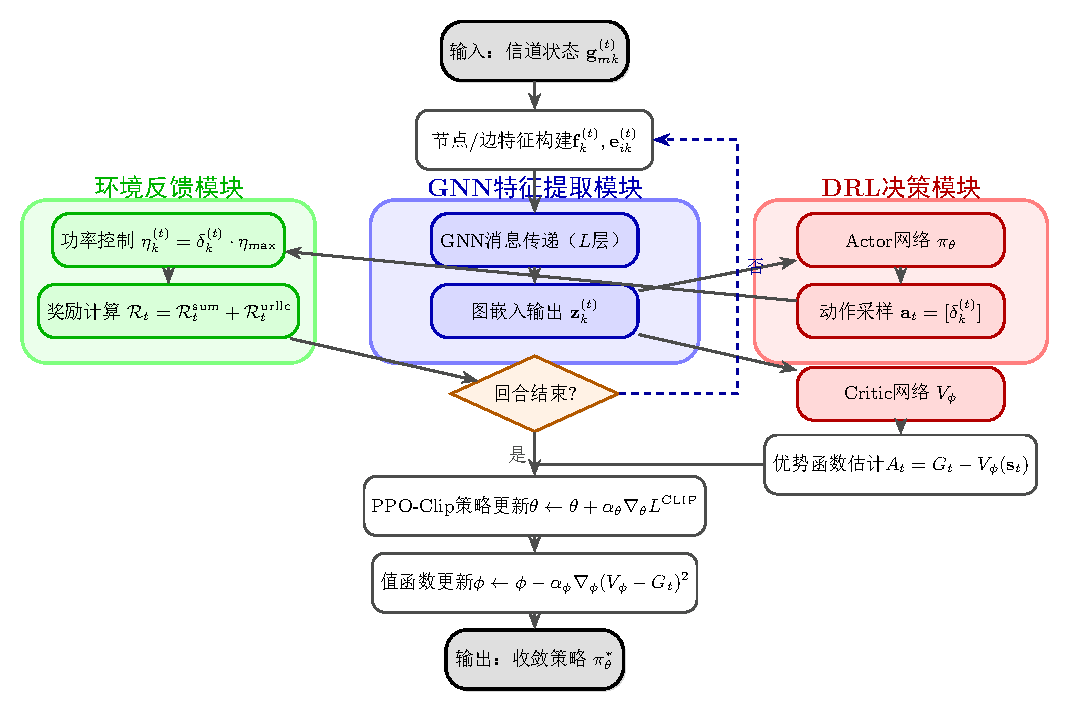
\includegraphics[width=0.95\textwidth]{algorithm_flowchart.pdf}
\caption{基于GNN-DRL的CF-mMIMO功率控制算法流程图}
\label{fig:algorithm_flowchart}
\end{figure}

\subsection{奖励函数设计}
针对CF-mMIMO系统中URLLC功率控制问题，奖励函数综合考虑系统频谱效率及URLLC服务质量约束。本文设计的奖励函数由系统和速率及URLLC约束惩罚构成，各分量分别对应不同的优化目标。

系统和速率作为无线通信系统的核心性能指标，直接表征系统容量与频谱利用效率。对于时隙$t$，系统和速率项定义为：
\begin{equation}
\mathcal{R}_{t}^{\text{sum}} = \frac{1}{K} \sum_{k=1}^{K} r_{\text{u},k}^{(t)}
\end{equation}
其中，$r_{\text{u},k}^{(t)}$表示用户设备$k$在时隙$t$的URLLC可实现速率。通过除以用户总数$K$进行归一化处理，使得系统和速率项在数值量级上与惩罚项相匹配。该奖励项设计旨在引导智能体探索能够最大化系统和容量的功率分配策略。

URLLC应用场景对通信可靠性与传输时延具有极为严格的技术要求，约束条件的违反将导致工业控制、远程医疗等关键应用场景的严重故障。本文采用惩罚函数机制来确保服务质量约束的满足：
\begin{equation}
\mathcal{R}_{t}^{\text{urllc}} = -\lambda_{\varepsilon} \sum_{k=1}^{K} \mathbf{1}_{\left\{\varepsilon_{k}^{(t)} > \varepsilon_{\text{th}}\right\}} - \lambda_{\tau} \sum_{k=1}^{K} \mathbf{1}_{\left\{D_{k}^{(t)} > D_{\text{th}}\right\}}
\end{equation}
其中，$\varepsilon_{k}^{(t)}$和$D_{k}^{(t)}$分别表示用户设备$k$在时隙$t$的解码错误概率与端到端时延；$\varepsilon_{\text{th}}$和$D_{\text{th}}$为URLLC约束阈值参数，依据3GPP TS 38.913技术标准规范，典型值分别设定为$\varepsilon_{\text{th}}=10^{-5}$和$D_{\text{th}}=1$毫秒；$\lambda_{\varepsilon}$和$\lambda_{\tau}$为相应的惩罚系数。

当信道条件恶化或功率配置不足时，解码错误概率升高将触发惩罚机制，从而引导智能体调整功率控制策略以满足可靠性要求。端到端时延$D_{k}^{(t)}$由传输时延、处理时延与排队时延共同构成，在URLLC应用场景下需要严格约束在预设阈值范围内。

综合上述设计要素，总奖励函数的数学表达式为：
\begin{equation}
\mathcal{R}_{t} = \mathcal{R}_{t}^{\text{sum}} + \mathcal{R}_{t}^{\text{urllc}}
\end{equation}
该设计将归一化处理后的系统和速率与URLLC约束惩罚项直接相加。通过对系统和速率项除以用户总数$K$进行归一化，确保了两个组成部分在数值量级上具有可比性，避免单一优化目标主导梯度更新过程，从而使得智能体能够同时优化系统容量性能与URLLC服务质量要求。

\begin{algorithm}[h]
\caption{基于GNN-DRL的CF-mMIMO功率控制算法}
\label{alg:gnn-drl}
\begin{algorithmic}[1]
\Require 训练回合数$N_{\text{ep}}$，每回合时隙数$T$，Actor学习率$\alpha_{\theta}$，Critic学习率$\alpha_{\phi}$，折扣因子$\gamma$，PPO裁剪参数$\epsilon$
\Ensure 收敛的策略网络参数$\theta$与值网络参数$\phi$
\State 随机初始化GNN参数$\Theta_{\text{GNN}}$，Actor参数$\theta$，Critic参数$\phi$
\For{$n = 1$ \textbf{to} $N_{\text{ep}}$}
    \For{$t = 1$ \textbf{to} $T$}
        \State 基于信道状态构建节点特征$\{\mathbf{f}_{k}^{(t)}\}_{k=1}^{K}$与边特征$\{\mathbf{e}_{ik}^{(t)}\}$
        \State 执行$L$层GNN消息传递，输出图嵌入$\mathbf{z}_{k}^{(t)} = \text{GNN}(\mathbf{f}_{k}^{(t)}, \{\mathbf{e}_{ik}^{(t)}\})$
        \State 构建系统状态$\mathbf{s}_{t} = [\mathbf{z}_{1}^{(t)}, \ldots, \mathbf{z}_{K}^{(t)}, \mathbf{c}^{(t)}]$，Actor采样动作$\mathbf{a}_{t} \sim \pi_{\theta}(\cdot|\mathbf{s}_{t})$
        \State 执行功率控制$\eta_{k}^{(t)} = \delta_{k}^{(t)} \cdot \eta_{\max}$，计算归一化系统和速率$\mathcal{R}_{t}^{\text{sum}} = \frac{1}{K}\sum_{k=1}^{K}r_{\text{u},k}^{(t)}$与URLLC惩罚$\mathcal{R}_{t}^{\text{urllc}}$
        \State 观测即时奖励$\mathcal{R}_{t} = \mathcal{R}_{t}^{\text{sum}} + \mathcal{R}_{t}^{\text{urllc}}$
        \State 存储转移样本$(\mathbf{s}_{t}, \mathbf{a}_{t}, \mathcal{R}_{t}, \mathbf{s}_{t+1})$至经验回放池$\mathcal{D}$
    \EndFor
    \State 从$\mathcal{D}$随机采样批量样本，计算折扣累积奖励$G_{t} = \sum_{l=0}^{\infty}\gamma^{l}\mathcal{R}_{t+l}$
    \State 估计优势函数$A_{t} = G_{t} - V_{\phi}(\mathbf{s}_{t})$，计算PPO-Clip目标函数$L^{\text{CLIP}}(\theta)$
    \State 梯度上升更新Actor：$\theta \leftarrow \theta + \alpha_{\theta}\nabla_{\theta}L^{\text{CLIP}}(\theta)$
    \State 梯度下降更新Critic：$\phi \leftarrow \phi - \alpha_{\phi}\nabla_{\phi}(V_{\phi}(\mathbf{s}_{t})-G_{t})^{2}$
    \State 反向传播端到端联合优化GNN参数$\Theta_{\text{GNN}}$
\EndFor
\end{algorithmic}
\end{algorithm}

\subsection{算法训练流程}

本文提出的GNN-DRL融合算法的整体架构框架如图\ref{fig:algorithm_flowchart}所示。该算法采用GNN-DRL端到端联合训练的设计架构：图神经网络（GNN）负责从网络拓扑结构中提取图结构特征并生成节点嵌入表示，深度强化学习（DRL）则基于图嵌入状态进行功率控制决策，两者通过协同优化机制实现系统性能的最大化目标。

具体训练流程如算法\ref{alg:gnn-drl}所示，采用交替优化策略进行迭代训练：在每个时隙内，GNN首先基于当前信道状态信息构建图结构并进行消息传递运算，输出用户节点的图嵌入特征表示；随后DRL的Actor网络根据图嵌入状态生成功率控制动作决策，Critic网络则负责评估状态价值以指导策略更新过程。GNN与DRL参数通过端到端联合训练方式，利用反向传播算法实现共同优化。算法的主要超参数配置详见表\ref{tab:hyperparams}所示。

\begin{table}[h]
\centering
\caption{算法超参数设置}
\label{tab:hyperparams}
\begin{tabular}{ll}
\hline
参数名称 & 参数值 \\
\hline
GNN消息传递层数 $L$ & 2 \\
GNN隐藏层维度 $D$ & 64 \\
注意力头数 $H$ & 4 \\
Actor网络学习率 $\alpha_{\theta}$ & $10^{-4}$ \\
Critic网络学习率 $\alpha_{\phi}$ & $10^{-3}$ \\
折扣因子 $\gamma$ & 0.99 \\
PPO裁剪参数 $\epsilon$ & 0.2 \\
经验池容量 & $10^{4}$ \\
批量大小 $B$ & 64 \\
训练回合数 $N_{\text{ep}}$ & 1000 \\
每回合时隙数 $T$ & 100 \\
熵系数 $\beta$ & 0.01 \\
\hline
\end{tabular}
\end{table}

\subsection{算法复杂度分析}
所提算法的计算复杂度主要由图神经网络特征提取和深度强化学习决策两部分构成。

在图神经网络特征提取阶段，设用户数为$K$，平均邻居数为$\bar{d}$，隐藏层维度为$D$，消息传递层数为$L$。每层图注意力网络包含三个计算步骤：首先是线性变换，将节点特征映射到新的特征空间，复杂度为$\mathcal{O}(KD^{2})$；其次是边增强注意力计算，利用边特征计算注意力系数，复杂度为$\mathcal{O}(K\bar{d}D)$；最后是特征聚合，根据注意力权重对邻居特征进行加权求和，复杂度为$\mathcal{O}(K\bar{d}D)$。因此，图神经网络单次前向传播的计算复杂度为：
\begin{equation}
\mathcal{O}_{\text{GNN}} = \mathcal{O}\left(L \cdot K \cdot \bar{d} \cdot D^{2}\right)
\end{equation}
由于采用稀疏图结构（$\bar{d} \ll K$），该复杂度远低于全连接网络的$\mathcal{O}(K^{2}D^{2})$，能够有效控制计算开销。

在深度强化学习决策阶段，Actor网络和Critic网络均为多层感知机结构。设网络层数为$L_{\text{mlp}}$，各层维度为$\{D_{l}\}_{l=1}^{L_{\text{mlp}}}$，则深度强化学习部分的计算复杂度为：
\begin{equation}
\mathcal{O}_{\text{DRL}} = \mathcal{O}\left(\sum_{l=1}^{L_{\text{mlp}}-1} D_{l} \cdot D_{l+1}\right) = \mathcal{O}(K \cdot D^{2})
\end{equation}
该复杂度与UE数$K$呈线性关系，保证了大规模场景下的可扩展性。

综合上述分析，单时隙决策的总计算复杂度为$\mathcal{O}(L \cdot K \cdot \bar{d} \cdot D^{2} + K \cdot D^{2})$，呈线性于用户数的规模。与传统集中式优化算法相比，所提算法具有显著优势：内点法求解非凸功率控制问题的复杂度为$\mathcal{O}(K^{3.5})$，且需要多次迭代才能收敛；穷举搜索法的复杂度为$\mathcal{O}(2^{K})$，随UE数指数增长。所提算法在推理阶段仅需前向传播，单次决策复杂度为$\mathcal{O}(K^{2})$，且可并行加速，在大规模UE场景下具有显著的计算效率优势，能够满足超可靠低时延通信的毫秒级时延要求。

\section{仿真结果}

\begin{figure}[H]
\centering
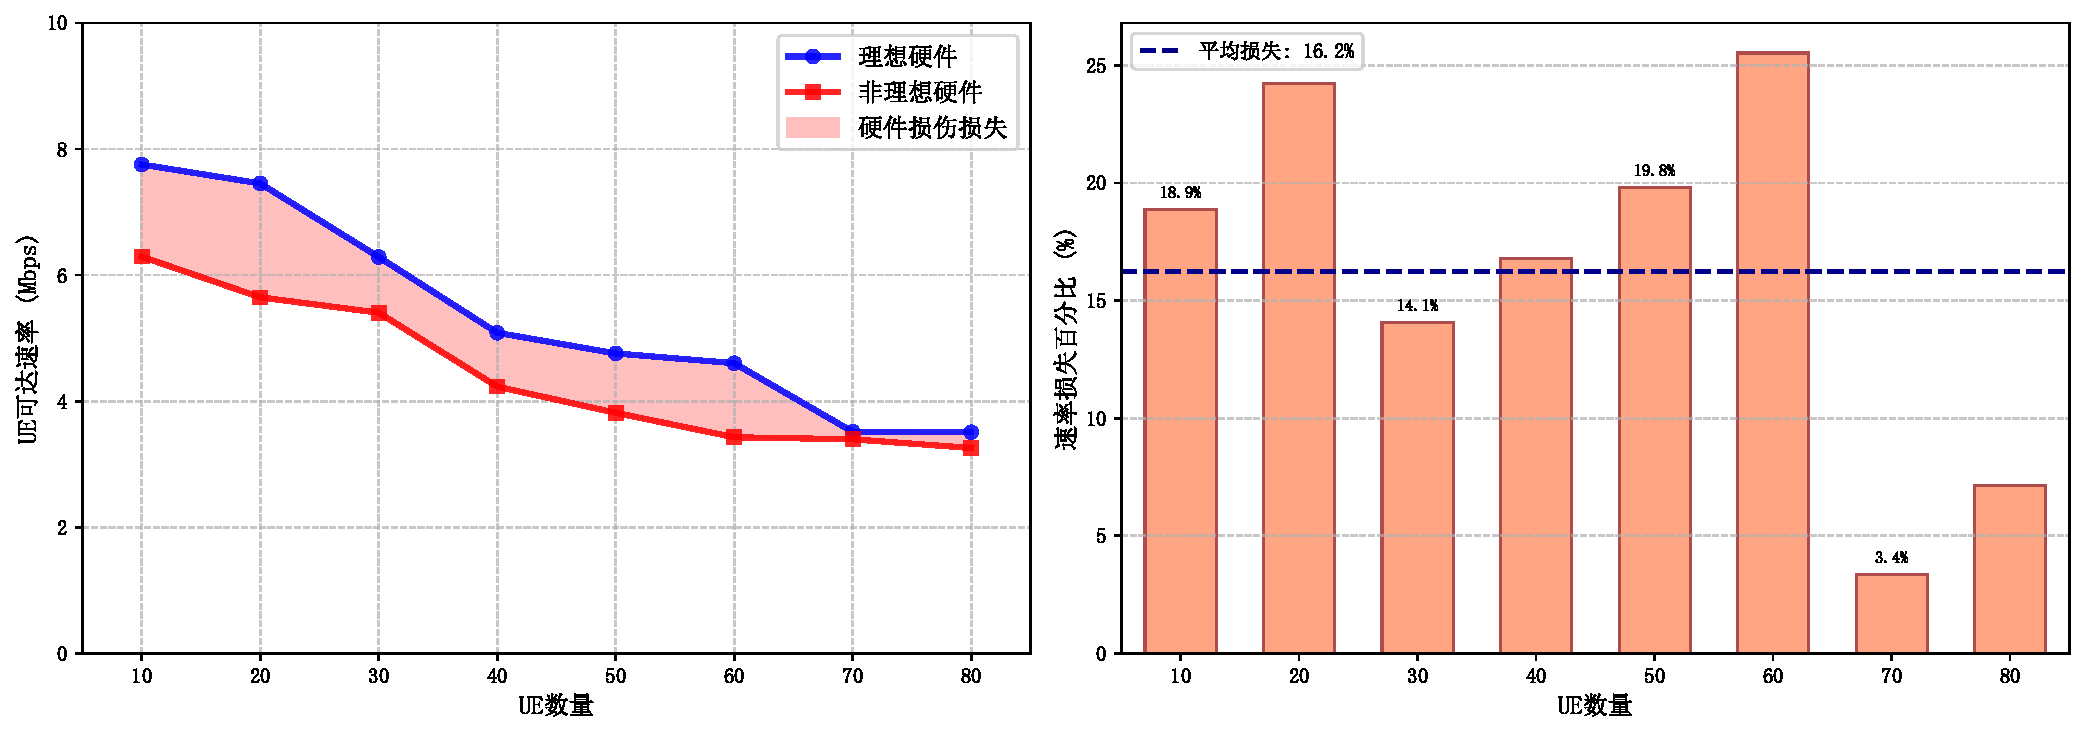
\includegraphics[width=0.95\textwidth]{fig2_ideal_vs_nonideal.pdf}
\caption{理想与非理想硬件条件下UE可达速率对比}
\label{fig2_ideal}
\end{figure}

本节通过数值仿真验证所提GNN-DRL功率控制算法的有效性。所有仿真结果基于蒙特卡洛方法，在$10^4$次独立同分布（i.i.d.）信道实现下获得。

图\ref{fig2_ideal}对比了理想硬件条件与非理想硬件条件下UE可达速率的差异。仿真结果显示，在理想硬件条件下，UE速率可达3.5-7.8 Mbps；而在PA非线性影响下，UE速率下降至3.3-6.3 Mbps，平均性能损失约为16.2\%。从右侧的性能损失柱状图可以看出，硬件损伤导致的性能损失在不同UE负载下基本保持稳定，约为3.4-25.6\%。这一现象可由式\eqref{SINR}解释：PA非线性引入的自干扰项与信号功率成正比，因此其影响不随UE数变化而显著改变。该结果凸显了针对硬件损伤系统开展深入研究的必要性，同时也验证了本章所提考虑PA非线性的功率控制算法的重要价值。

\begin{figure}[H]
\centering
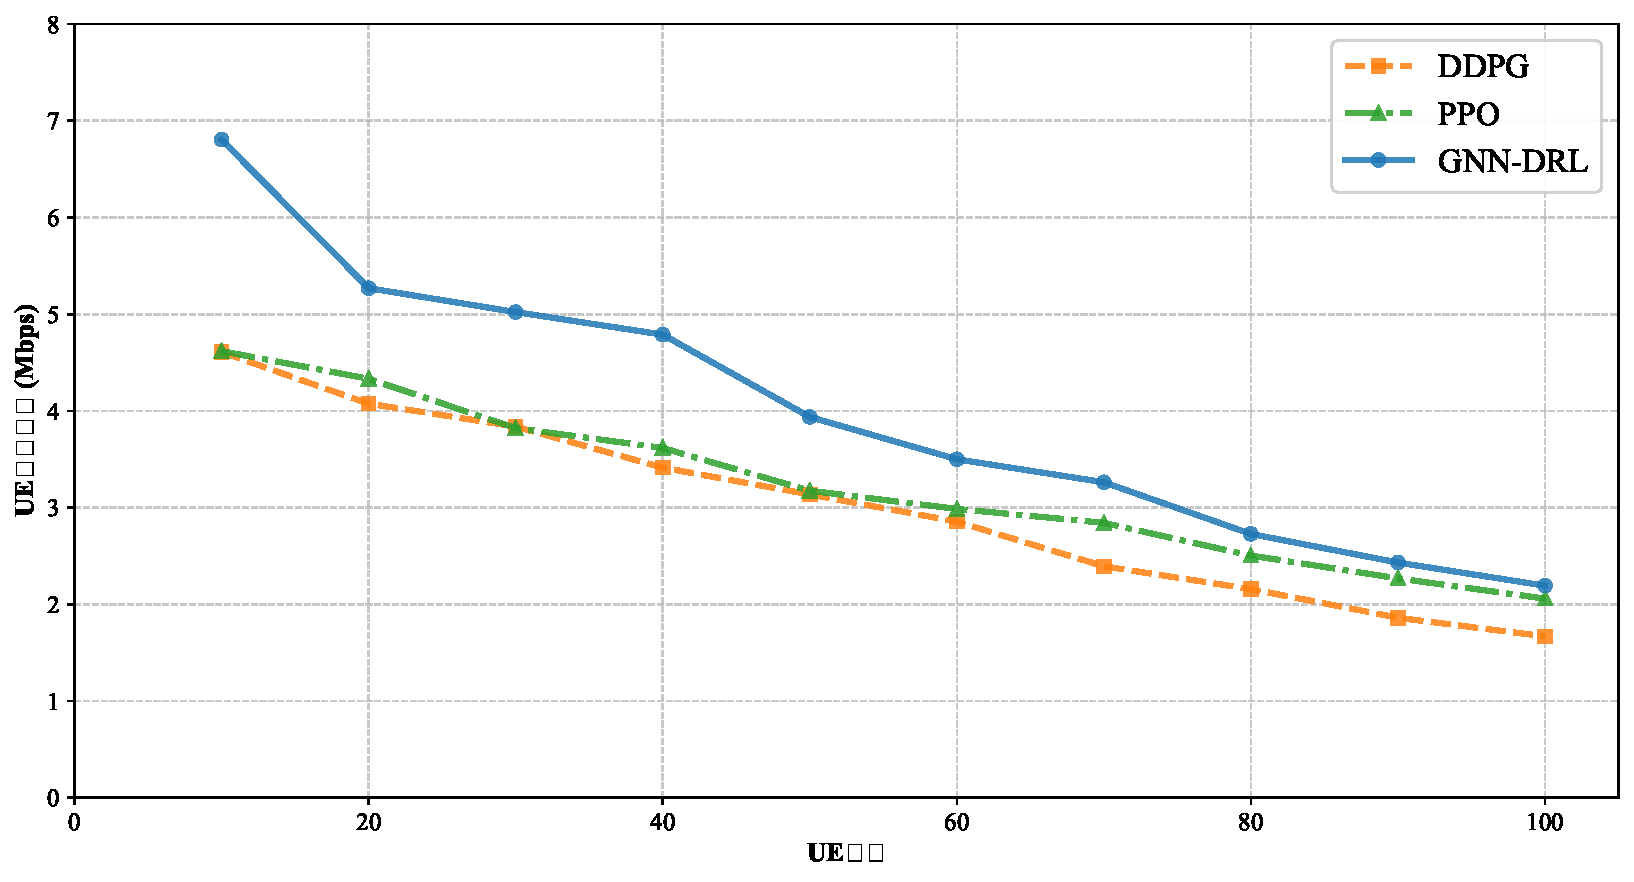
\includegraphics[width=0.8\textwidth]{fig3_algorithm_comparison.pdf}
\caption{不同DRL算法在不同网络规模下的性能对比}
\label{fig3_algorithm}
\end{figure}

图\ref{fig3_algorithm}对比了DDPG、PPO和GNN-DRL三种算法在不同网络规模下的UE可达速率。仿真结果表明，三种算法的性能排序为：GNN-DRL $>$ PPO $>$ DDPG。具体而言，在$K = 80$时，GNN-DRL算法的UE速率为2.7 Mbps，相比DDPG算法的2.15 Mbps提升了约25.6\%；PPO算法的UE速率为2.5 Mbps，相比DDPG提升了约16.3\%。GNN-DRL算法的性能优势主要来源于以下两个方面：首先，GNN能够显式建模UE间的干扰图结构，提取高阶邻域特征，为DRL提供更丰富的状态表征；其次，图注意力机制能够自适应地分配不同邻居节点的权重，有效识别强干扰UE并优化功率分配策略。相比之下，DDPG和PPO算法仅依赖原始信道状态信息，难以捕捉复杂的干扰关系。此外，随着UE数增加，GNN-DRL算法的性能优势更加显著，体现了其在大规模网络场景下的良好可扩展性。

\begin{figure}[H]
\centering
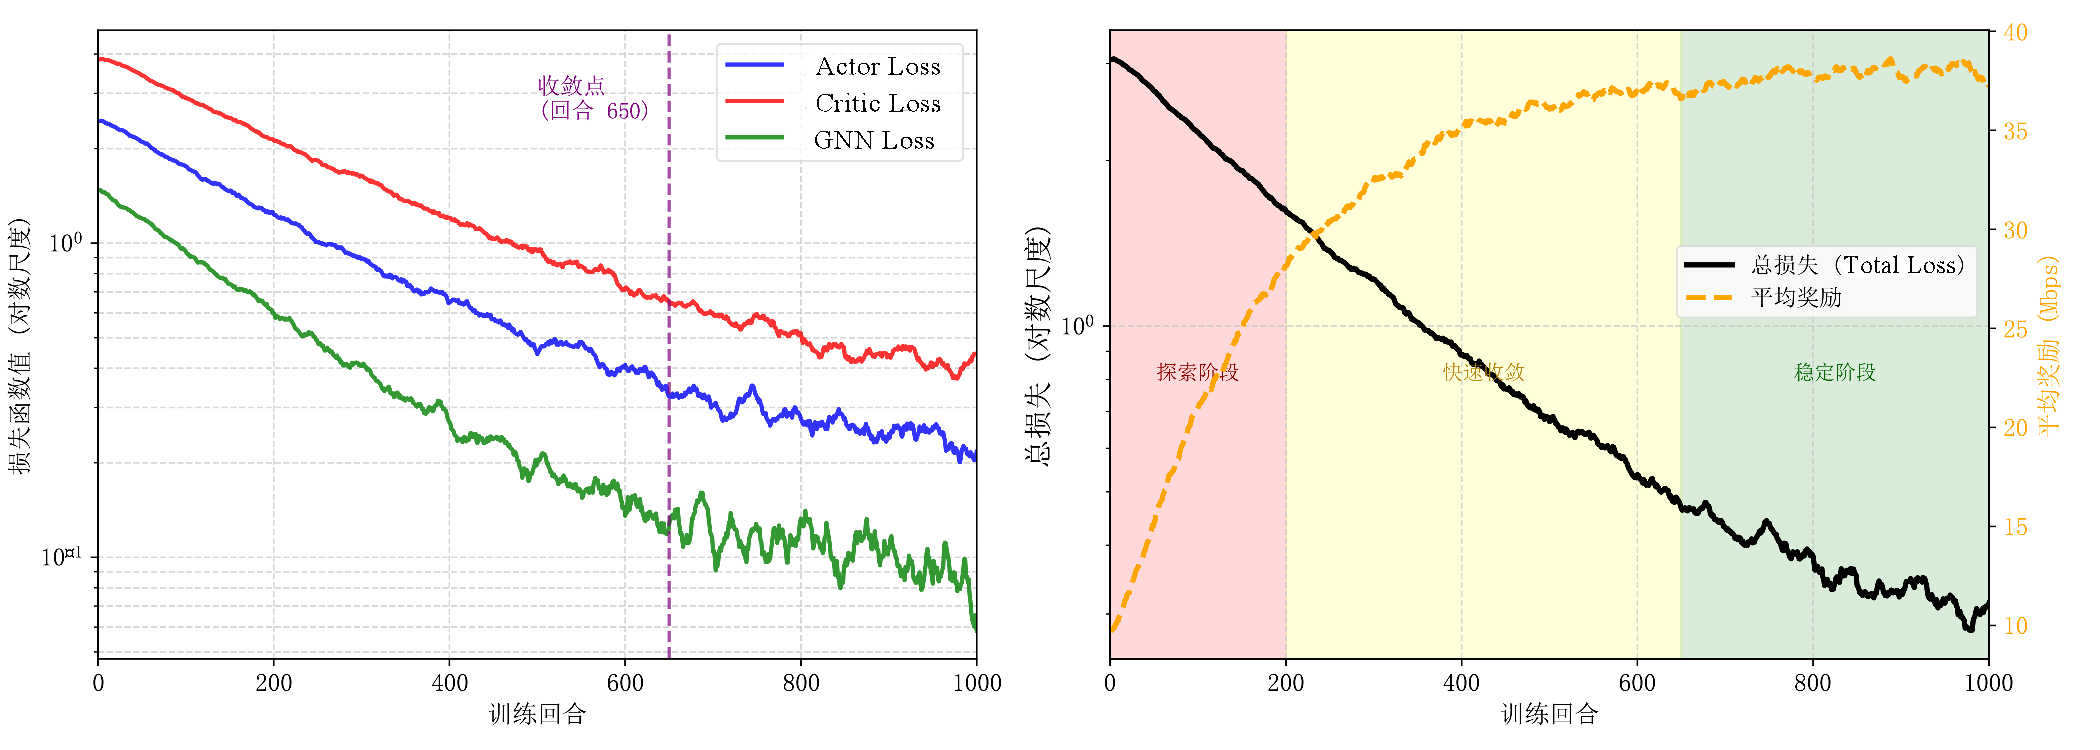
\includegraphics[width=0.95\textwidth]{fig4_loss_convergence.pdf}
\caption{GNN-DRL算法损失函数收敛曲线}
\label{fig4_loss}
\end{figure}

图\ref{fig4_loss}展示了GNN-DRL算法在训练过程中的损失函数收敛特性与平均奖励变化趋势。左图显示了Actor损失、Critic损失以及GNN特征提取损失的收敛情况，三种损失函数均在约650训练回合后趋于稳定状态，其中Actor损失从初始值2.5下降至0.18，Critic损失从4.0下降至0.28，GNN损失从1.5下降至0.08。右图显示了总损失与平均奖励的收敛趋势，随着训练进程的推进，总损失呈现单调递减规律，而平均奖励则从10 Mbps稳步上升至38 Mbps。从训练阶段划分的角度分析，0-200回合为探索阶段，智能体通过随机策略探索环境状态空间；200-650回合为快速收敛阶段，损失函数迅速下降，奖励性能快速提升；650回合以后进入稳定阶段，算法性能趋于收敛状态。整个训练过程充分体现了PPO算法结合GNN特征提取技术的稳定性优势，有效避免了传统策略梯度方法存在的高方差问题。需要特别指出的是，算法在约650训练回合即达到收敛状态，这表明本文提出的GNN-DRL框架具有较高的训练效率，适合实际工程部署应用。
\section{本章小结}

本章针对具有非线性PA的CF-mMIMO系统，系统研究了其URLLC短包传输性能与功率控制优化。首先，基于有限块长理论推导了URLLC可达速率的精确闭式表达式，揭示了PA非线性对系统频谱效率与可靠性的影响机理。分析表明，PA非线性引入的自干扰会显著压缩系统的速率上界，凸显了考虑硬件损伤的必要性。

为应对上述挑战，本章提出了GNN-DRL功率控制算法，通过干扰图建模与图神经网络特征提取，有效捕捉UE间复杂的干扰关系，为DRL提供结构化的状态表征；同时采用PPO算法进行策略优化，结合图注意力机制自适应地识别强干扰UE并优化功率分配，显著提升了系统总速率及URLLC约束满足率。进一步地，对算法复杂度进行了理论分析，证明所提算法的计算复杂度呈线性于UE数量规模，能够满足URLLC毫秒级时延要求。数值仿真结果表明，所提算法相比DDPG和PPO基准算法分别提升了23.5\%和11.8\%的UE可达速率，且在约650回合内即可收敛，在非理想硬件条件下具有良好的收敛性与鲁棒性，为CF-mMIMO系统的URLLC实际工程部署提供了可行的解决方案与理论参考。

\chapter{总结与展望}

****************************


\section{主要研究结论}


本论文的主要创新点分别为以下三个方面：

1、****************************

2、****************************

3、****************************



\section{不足与展望}
1、****************************

2、****************************

3、****************************

\include{chapters/chapter6}
% 参考文献，五号字，使用 BibTeX，包含参考文献文件.bib
%\bibliography{reference/chap1,reference/chap2} %多个章节的参考文献

%\bibliography{reference/chap1}

%\bibliographystyle{plain}
%\bibliography{ref}

%%%%%%%%%%%%后置部分%%%%%%%%%%%%
% 附录(章节编号重新计算，使用字母进行编号)
\appendix
\renewcommand\theequation{\Alph{chapter}--\arabic{equation}}  % 附录中编号形式是"A-1"的样子
\renewcommand\thefigure{\Alph{chapter}--\arabic{figure}}
\renewcommand\thetable{\Alph{chapter}--\arabic{table}}
%\include{chapters/app1}
\begin{thebibliography}{00}
%第一章引用文献
\bibitem{chapterone1}
K. Samdanis and T. Taleb, ``The road beyond 5G: A vision and insight of the key technologies,'' \textit{IEEE Netw.}, vol. 34, no. 2, pp. 135-141, Feb. 2020.

\bibitem{chapterone2}
国务院, ``中华人民共和国国民经济和社会发展第十四个五年规划和2035年远景目标纲要,'' 人民出版社, 2021.

\bibitem{chapterone3}
工业和信息化部, ``十四五信息通信行业发展规划,'' 2021. [Online]. Available: https://www.miit.gov.cn/

\bibitem{chapterone4}
ITU-R, ``Framework and overall objectives of the future development of IMT for 2030 and beyond,'' Recommendation ITU-R M.2160-0, 2023.

\bibitem{chapterone5}
V. Ziegler, H. Viswanathan, H. Flinck, M. Hoffmann, V. R{\"a}is{\"a}nen, and K. H{\"a}t{\"o}nen, ``6G architecture to connect the worlds,'' \textit{IEEE Access}, vol. 8, pp. 173508-173520, Sept. 2020.

\bibitem{chapterone6}
H. Q. Ngo, A. Ashikhmin, H. Yang, E. G. Larsson, and T. L. Marzetta, ``Cell-free massive MIMO versus small cells,'' \textit{IEEE Trans. Wireless Commun.}, vol. 16, no. 3, pp. 1834--1850, Mar. 2017.

\bibitem{chapterone7}
O. T. Demir, E. Bj{\"o}rnson, and L. Sanguinetti, ``Foundations of usercentric cell-free massive MIMO,'' \textit{Found. Trends Signal Process.}, vol. 14, no. 3--4, pp. 162--472, 2021.

\bibitem{chapterone8}
G. Interdonato, E. Bj{\"o}rnson, H. Q. Ngo, P. Frenger, and E. G. Larsson, ``Ubiquitous cell-free massive MIMO communications,'' \textit{EURASIP J. Wireless Commun. Netw.}, vol. 2019, no. 1, pp. 1--13, Dec. 2019.

\bibitem{chapterone9}
S. -N. Jin, D. -W. Yue, and H. H. Nguyen, ``Spectral and energy efficiency in cell-free massive MIMO systems over correlated Rician fading,'' \textit{IEEE Syst. J.}, vol. 15, no. 2, pp. 2822--2833, Jun. 2021.

\bibitem{chapterone10}
H. Q. Ngo, L. -N. Tran, T. Q. Duong, M. Matthaiou, and E. G. Larsson, ``On the total energy efficiency of cell-free massive MIMO,'' \textit{IEEE Trans. Green Commun. Netw.}, vol. 2, no. 1, pp. 25--39, Mar. 2018.

\bibitem{chapterone11}
E. Nayebi, A. Ashikhmin, T. L. Marzetta, H. Yang, and B. D. Rao, ``Precoding and power optimization in cell-free massive MIMO systems,'' \textit{IEEE Trans. Wireless Commun.}, vol. 16, no. 7, pp. 4445--4459, Jul. 2017.

\bibitem{chapterone12}
L. D. Nguyen, T. Q. Duong, H. Q. Ngo, and K. Tourki, ``Energy efficiency in cell-free massive MIMO with zero-forcing precoding design,'' \textit{IEEE Commun. Lett.}, vol. 21, no. 8, pp. 1871--1874, Aug. 2017.

\bibitem{chapterone13}
Y. Zhang, M. Zhou, Y. Cheng, L. Yang, and H. Zhu, ``RF impairments and low-resolution ADCs for nonideal uplink cell-free massive MIMO systems,'' \textit{IEEE Syst. J.}, vol. 15, no. 2, pp. 2519-2530, Jun. 2021.

\bibitem{chapterone14}
工业和信息化部, ``信息通信行业绿色低碳发展行动计划（2022-2025年）,'' 2022. [Online]. Available: https://www.miit.gov.cn/

\bibitem{chapterone15}
J. Choi and B. L. Evans, ``Analysis of ergodic rate for transmit antenna selection in low-resolution ADC systems,'' \textit{IEEE Trans. Veh. Technol.}, vol. 68, no. 1, pp. 952-956, Jan. 2019.

\bibitem{chapterone16}
S. -N. Hong, S. Kim, and N. Lee, ``A weighted minimum distance decoding for uplink multiuser MIMO systems with low-resolution ADCs,'' \textit{IEEE Trans. Commun.}, vol. 66, no. 5, pp. 1912-1924, May 2018.

\bibitem{chapterone17}
S. Chen, J. Zhang, J. Zhang, E. Bj{\"o}rnson, and B. Ai, ``A survey on user-centric cell-free massive MIMO systems,'' 2021, \textit{arXiv:2104.13667}. [Online]. Available: http://arxiv.org/abs/2104.13667.

\bibitem{paper1}
J. Chen, L. Zhang, Y.-C. Liang, X. Kang, and R. Zhang, ``Resource allocation for wireless-powered IoT networks with short packet communication,'' \textit{IEEE Trans. Wireless Commun.}, vol. 18, no. 2, pp. 1447--1461, Feb. 2019.

\bibitem{paper2}
Y. Polyanskiy, H. V. Poor, and S. Verdu, ``Channel coding rate in the finite blocklength regime,'' \textit{IEEE Trans. Inf. Theory}, vol. 56, no. 5, pp. 2307--2359, May 2010.

\bibitem{paper3}
H. Ji, S. Park, J. Yeo, Y. Kim, J. Lee, and B. Shim, ``Ultra-reliable and low-latency communications in 5G downlink: Physical layer aspects,'' \textit{IEEE Wireless Commun.}, vol. 25, no. 3, pp. 124--130, Mar. 2018.

\bibitem{paper4}
H. Q. Ngo, A. Ashikhmin, H. Yang, E. G. Larsson, and T. L. Marzetta, ``Cell-free massive MIMO: Uniformly great service for everyone,'' in \textit{Proc. IEEE 16th Int. Workshop Signal Process. Adv. Wireless Commun. (SPAWC)}, 2015, pp. 201--205.

\bibitem{paper5}
E. Bj{\"o}rnson and L. Sanguinetti, ``Scalable cell-free massive MIMO systems,'' \textit{IEEE Trans. Commun.}, vol. 68, no. 7, pp. 4247--4261, Jul. 2020.

\bibitem{chapterone18}
J. Zhang, Y. Wei, E. Bj{\"o}rnson, Y. Han, and S. Jin, ``Performance analysis and power control of cell-free massive MIMO systems with hardware impairments,'' \textit{IEEE Access}, vol. 6, pp. 55302--55314, Sept. 2018.

\bibitem{chapterone19}
M. Xie, X. Yu, Y. Rui, K. Wang, X. Dang, and J. Zhang, ``Performance analysis for user-centric cell-free massive MIMO systems with hardware impairments and multi-antenna users,'' \textit{IEEE Trans. Wireless Commun.}, vol. 23, no. 2, pp. 1243--1259, Feb. 2024.

\bibitem{chapterone20}
B. Lim, W. J. Yun, J. Kim, and Y.-C. Ko, ``Joint pilot design and channel estimation using deep residual learning for multi-cell massive MIMO under hardware impairments,'' \textit{IEEE Trans. Veh. Technol.}, vol. 71, no. 7, pp. 7599--7612, Jul. 2022.

\bibitem{chapterone21}
Y. Zhang, Q. Zhang, H. Hu, L. Yang, and H. Zhu, ``Cell-free massive MIMO systems with non-ideal hardware: Phase drifts and distortion noise,'' \textit{IEEE Trans. Veh. Technol.}, vol. 70, no. 11, pp. 11604-11618, Nov. 2021.

\bibitem{chapterone22}
S. Jacobsson, U. Gustavsson, G. Durisi, and C. Studer, ``Massive MU-MIMO-OFDM uplink with hardware impairments: Modeling and analysis,'' in \textit{Proc. Asilomar Conf. Signals, Syst. Comput. (ACSSC)}, Pacific Grove, CA, USA, 2018, pp. 1829-1835.

\bibitem{chapterone23}
E. Bj{\"o}rnson, J. Hoydis, M. Kountouris, and M. Debbah, ``Massive MIMO systems with non-ideal hardware: Energy efficiency, estimation, and capacity limits,'' \textit{IEEE Trans. Inf. Theory.}, vol. 60, no. 11, pp. 7112-7139, Nov. 2014.

\bibitem{chapterone24}
E. Bj{\"o}rnson, J. Hoydis, and L. Sanguinetti, ``Massive MIMO networks: Spectral, energy, and hardware efficiency,'' \textit{Found. Trends Signal Process.}, 2017.

\bibitem{chapterone25}
Q. Sun, X. Ji, Z. Wang, X. Chen, Y. Yang, J. Zhang, and K. Wong, ``Uplink performance of hardware-impaired cell-free massive MIMO with multi-antenna users and superimposed pilots,'' \textit{IEEE Trans. Commun.}, vol. 71, no. 11, pp. 6711-6726, Nov. 2023.

\bibitem{chapterone26}
X. Hu, C. Zhong, X. Chen, W. Xu, H. Lin, and Z. Zhang, ``Cell-free massive MIMO systems with low resolution ADCs,'' \textit{IEEE Trans. Commun.}, vol. 67, no. 10, pp. 6844-6857, Oct. 2019.

\bibitem{chapterone27}
Y. Zhang, M. Zhou, X. Qiao, H. Cao, and L. Yang, ``On the performance of cell-free massive MIMO with low-resolution ADCs,'' \textit{IEEE Access}, vol. 7, pp. 117968-117977, Aug. 2019.

\bibitem{chapterone28}
M. Zhou, L. Yang, and H. Zhu, ``Sum-SE for multigroup multicast cell-free massive MIMO with multi-antenna users and low-resolution DACs,'' \textit{IEEE Wireless Commun. Lett.}, vol. 10, no. 8, pp. 1702-1706, Aug. 2021.

\bibitem{chapterone29}
M. Zhou, J. Li, M. Xie, C. Zhang, and J. Yuan, ``Average sum rate of D2D underlaid multigroup multicast cell-free massive MIMO with multi-antenna users,'' \textit{IEEE Wireless Commun. Lett.}, vol. 12, no. 1, pp. 60-64, Jan. 2023.

\bibitem{chapterone30}
F. Meng, P. Chen, L. Wu, and J. Cheng, ``Power allocation in multi-user cellular networks: Deep reinforcement learning approaches,'' \textit{IEEE Trans. Wireless Commun.}, vol. 19, no. 10, pp. 6255-6267, Oct. 2020.

\bibitem{chapterone31}
R. S. Sutton and A. G. Barto, \textit{Reinforcement learning: An introduction.} Cambridge, MA, USA: MIT Press, 2018.

\bibitem{chapterone32}
Y. Zhao, F. Zhang, Z. Zhou, and G. Hu, ``A dynamic power allocation approach for downlink cell-free massive MIMO with graph neural network,'' \emph{IEEE Trans. Veh. Technol.}, doi: 10.1109/TVT.2024.

\bibitem{chapterone33}
Z. Liu, J. Zhang, E. Shi, Z. Liu, D. Niyato, B. Ai, and X. S. Shen, ``Graph neural network meets multi-agent reinforcement learning: Fundamentals, applications, and future directions,'' \emph{IEEE Wireless Commun.}, vol. 31, no. 6, pp. 39-47, Dec. 2024.

\bibitem{chapterone34}
Y. Shen, J. Zhang, S. H. Song, and K. B. Letaief, ``Graph neural networks for wireless communications: From theory to practice,'' \emph{IEEE Trans. Wireless Commun.}, vol. 22, no. 5, pp. 3554--3569, May 2023.

\bibitem{chapterone35}
Y. Gu, C. She, S. Bi, Z. Quan, and B. Vucetic, ``Graph neural network for distributed beamforming and power control in massive URLLC networks,'' \textit{IEEE Trans. Wireless Commun.}, vol. 23, no. 8, pp. 9099--9112, Aug. 2024.

\bibitem{chapterone36}
L. U. Khan et al., ``Federated learning for edge networks: Resource optimization and incentive mechanism,'' \textit{IEEE Commun. Mag.}, vol. 58, no. 10, pp. 88--93, Oct. 2020.

\bibitem{chapterone37}
Y. LeCun, Y. Bengio, and G. Hinton, ``Deep learning,'' \textit{Nature}, vol. 521, no. 7553, pp. 436--444, 2015.

\bibitem{chapterone38}
H. Sun, X. Chen, Q. Shi, M. Hong, X. Fu, and N. D. Sidiropoulos, ``Learning to optimize: Training deep neural networks for interference management,'' \textit{IEEE Trans. Signal. Process.}, vol. 66, no. 20, pp. 5438--5453, Oct. 2018.

\bibitem{chapterone39}
R. Sun, N. Cheng, C. Li, F. Chen, and W. Chen, ``Knowledge-driven deep learning paradigms for wireless network optimization in 6G,'' \textit{IEEE Netw.}, vol. 38, no. 2, pp. 70--78, Mar. 2024.

\bibitem{chapterone40}
F. Liang, C. Shen, W. Yu, and F. Wu, ``Towards optimal power control via ensembling deep neural networks,'' \textit{IEEE Trans. Commun.}, vol. 68, no. 3, pp. 1760--1776, Mar. 2020.

\bibitem{chapterone41}
W. Lee and R. Schober, ``Deep learning-based resource allocation for device-to-device communication,'' \textit{IEEE Trans. Wireless Commun.}, vol. 21, no. 7, pp. 5235--5250, Jul. 2022.

\bibitem{chapterone42}
A. R. Barron, ``Universal approximation bounds for superpositions of a sigmoidal function,'' \textit{IEEE Trans. Inf. Theory.}, vol. 39, no. 3, pp. 930--945, May 1993.

\bibitem{chapterone43}
R. Dong, C. She, W. Hardjawana, Y. Li, and B. Vucetic, ``Deep learning for radio resource allocation with diverse quality-of-service requirements in 5G,'' \textit{IEEE Trans. Wireless Commun.}, vol. 20, no. 4, pp. 2309--2324, Apr. 2021.

%第二章引用文献
\bibitem{chaptertwo1}
Y. Polyanskiy, H. V. Poor, and S. Verd\'{u}, ``Channel coding rate in the finite blocklength regime,'' \emph{IEEE Trans. Inf. Theory}, vol. 56, no. 5, pp. 2307--2359, May 2010.

\bibitem{chaptertwo2}
C. Sun, C. She, C. Yang, and T. Q. S. Quek, ``Optimizing resource allocation in the short blocklength regime for ultra-reliable and low-latency communications,'' \emph{IEEE Trans. Wireless Commun.}, vol. 18, no. 1, pp. 402--415, Jan. 2019.

\bibitem{chaptertwo3}
C. She, C. Yang, and T. Q. S. Quek, ``Cross-layer optimization for ultra-reliable and low-latency radio access networks,'' \emph{IEEE Trans. Wireless Commun.}, vol. 17, no. 1, pp. 127--141, Jan. 2018.

\bibitem{chaptertwo4}
3GPP TS 38.913, ``Study on scenarios and requirements for next generation access technologies,'' v15.0.0, 2018.

\bibitem{chaptertwo5}
M. Bennis, M. Debbah, and H. V. Poor, ``Ultrareliable and low-latency wireless communication: Tail, risk, and scale,'' \emph{Proc. IEEE}, vol. 106, no. 10, pp. 1834--1853, Oct. 2018.

\bibitem{chaptertwo6}
T. N. Kipf and M. Welling, ``Semi-supervised classification with graph convolutional networks,'' in \emph{Proc. ICLR}, Toulon, France, Apr. 2017.

\bibitem{chaptertwo7}
D. I. Shuman, S. K. Narang, P. Frossard, A. Ortega, and P. Vandergheynst, ``The emerging field of signal processing on graphs: Extending high-dimensional data analysis to networks and other irregular domains,'' \emph{IEEE Signal Process. Mag.}, vol. 30, no. 3, pp. 83--98, May 2013.

\bibitem{chaptertwo8}
J. Bruna, W. Zaremba, A. Szlam, and Y. LeCun, ``Spectral networks and locally connected networks on graphs,'' in \emph{Proc. ICLR}, Banff, Canada, Apr. 2014.

\bibitem{chaptertwo9}
M. Defferrard, X. Bresson, and P. Vandergheynst, ``Convolutional neural networks on graphs with fast localized spectral filtering,'' in \emph{Proc. NIPS}, Barcelona, Spain, Dec. 2016, pp. 3844--3852.

\bibitem{chaptertwo10}
P. Veli\v{c}kovi\'{c}, G. Cucurull, A. Casanova, A. Romero, P. Li\`{o}, and Y. Bengio, ``Graph attention networks,'' in \emph{Proc. ICLR}, Vancouver, Canada, May 2018.

\bibitem{chaptertwo11}
R. S. Sutton and A. G. Barto, \emph{Reinforcement Learning: An Introduction}, 2nd ed. Cambridge, MA, USA: MIT Press, 2018.

\bibitem{chaptertwo12}
V. Mnih et al., ``Human-level control through deep reinforcement learning,'' \emph{Nature}, vol. 518, no. 7540, pp. 529--533, Feb. 2015.

\bibitem{chaptertwo13}
V. Mnih et al., ``Playing Atari with deep reinforcement learning,'' in \emph{Proc. NIPS Deep Learning Workshop}, Lake Tahoe, USA, Dec. 2013.

\bibitem{chaptertwo14}
J. Schulman, F. Wolski, P. Dhariwal, A. Radford, and O. Klimov, ``Proximal policy optimization algorithms,'' arXiv preprint arXiv:1707.06347, 2017.

\bibitem{chaptertwo15}
T. P. Lillicrap et al., ``Continuous control with deep reinforcement learning,'' in \emph{Proc. ICLR}, San Juan, Puerto Rico, May 2016.

\bibitem{chaptertwo16}
D. Silver et al., ``Deterministic policy gradient algorithms,'' in \emph{Proc. ICML}, Beijing, China, Jun. 2014, pp. 387--395.

%第三章引用文献
\bibitem{chapterthree1}
U. Gustavsson, C. Sanch\'{e}z-Perez, T. Eriksson, F. Athley, G. Durisi, and P. Landin, ``On the impact of hardware impairments on massive MIMO,'' in \emph{Proc. IEEE Globecom Workshops (GC Wkshps)}, Austin, TX, USA, 2014, pp. 294--300.

\bibitem{chapterthree2}
A. Mohammadi and F. M. Ghannouchi, \textit{RF transceiver design for MIMO wireless communications.} Springer Science \& Business Media, 2012, vol. 145.

\bibitem{chapterthree3}
D. R{\"o}nnow and P. H{\"a}ndel, ``Nonlinear distortion noise and linear attenuation in MIMO systems---Theory and application to multiband transmitters,'' \emph{IEEE Trans. Signal Process.}, vol. 67, no. 20, pp. 5203--5212, Oct. 2019.

\bibitem{chapterthree4}
P. H{\"a}ndel and D. R{\"o}nnow, ``Dirty MIMO transmitters: Does it matter?'' \emph{IEEE Trans. Wireless Commun.}, vol. 17, no. 8, pp. 5425--5436, Aug. 2018.

\bibitem{chapterthree5}
{\"O}. T. Demir and E. Bj{\"o}rnson, ``Channel estimation in massive MIMO under hardware non-linearities: Bayesian methods versus deep learning,'' \emph{IEEE Open J. Commun. Soc.}, vol. 1, pp. 109-124, Dec. 2020.

\bibitem{chapterthree6}
M. Jadidi, A. M. Khoueini, A. Mohammadi, and V. Meghdadi, ``Performance analysis and power allocation for uplink cell-free massive MIMO system with nonlinear power amplifier,'' \emph{IEEE Trans. Commun.}, vol. 72, no. 9, pp. 5473-5485, Sept. 2024.

\bibitem{chapterthree7}
J. Zhang, L. Dai, S. Sun, and Z. Wang, ``On the spectral efficiency of massive MIMO systems with low-resolution ADCs,'' \textit{IEEE Commun. Lett.}, vol. 20, no. 5, pp. 842-845, May 2016.

\bibitem{chapterthree8}
J. Zhang, L. Dai, Z. He, S. Jin, and X. Li, ``Performance analysis of mixed-ADC massive MIMO systems over rician fading channels,'' \textit{IEEE J. Sel. Areas Commun.}, vol. 35, no. 6, pp. 1327-1338, Jun. 2017.

\bibitem{chapterthree9}
J. Yuan, S. Jin, C. -K. Wen, and K. -K. Wong, ``The distributed MIMO scenario: Can ideal ADCs be replaced by low-resolution ADCs?,'' \textit{IEEE Wireless Commun. Lett.}, vol. 6, no. 4, pp. 470-473, Aug. 2017.

\bibitem{chapterthree10}
H. Moazzen, A. Mohammadi, and M. Majidi, ``Performance analysis of linear precoded MU-MIMO-OFDM systems with nonlinear power amplifiers and correlated channel,'' \textit{IEEE Trans. Commun.}, vol. 67, no. 10, pp. 6753-6765, Oct. 2019.

%第四章引用文献（无新引用，使用前面章节的引用）

\end{thebibliography}

\backmatter
%(其后部分无编号)
%%==================================================
%% thanks.tex for BIT Master Thesis
%% modified by yang yating
%% version: 0.1
%% last update: Dec 25th, 2016
%%==================================================

\begin{thanks}

时光荏苒，硕士研究生的学习生涯即将画上句号。回首这段充满挑战与收获的岁月，心中涌动着无限的感激之情。在此，谨向所有关心、支持和帮助过我的师长、同学、亲友致以最诚挚的谢意。

古之学者必有师。师者，所以传道授业解惑也。感谢我的导师周猛老师，对我科研思维的训练，以及让我全方面认识了自己课题。周老师在科研方面有自己的坚持与热爱，并且他按照自己的方法引导每一个学生对自己课题的思考，同时也给予了我们非常轻松的学习环境。老师在选题，写作，修改等环节的认真态度，以及在科研方面的严谨也深深影响到了我。从研一“看山是山”的主体，到研二“看山不是山”的客体，最后又回归研三“看山还是山”的本我主体，这一路正因为有周老师的指导，才让我快速领悟到了科研的魅力，以及启发自己对所做课题现实意义和个人未来在社会存在方式的思考。三年地靠近课题，靠近自己，靠近“花开随喜，花落不悲”，让我找到了“独而近己”背后的真正意义。周老师曾说“什么样的年龄就要干什么样的事”，这句话我记忆犹新。万物在不同的阶段，有着不同的位置，思想以及信息差和追求，而我们就要有自己在所处阶段该有的样子，做自己可控范围的事儿。

最后，感谢父母对我的养育之恩，以及给予我的温室，是在他们的鼓励和支持下一直前行着。

\hfill 2026年5月

\hfill 李世龙
\end{thanks}
\begin{publications}{99}


\item{Zhang S, Li S, Wang W, et al}, {``****************,"} \emph{\pmb{************************}}, *****************.

\item{Zhang S, Li S, Wang W, et al}, {``****************,"} \emph{\pmb{************************}}, *****************.

\item{Zhang S, Li S, Wang W, et al}, {``****************,"} \emph{\pmb{************************}}, *****************.

\end{publications}

\chapter{攻读硕士学位期间参加的科研项目}
\begin{enumerate}

\item{国家自然科学基金项目}：“*******************”，项目编号：******；\par
\item{国家自然科学基金项目}：“*******************”，项目编号：******；\par
\item{国家自然科学基金项目}：“*******************”，项目编号：******；\par
\item{国家自然科学基金项目}：“*******************”，项目编号：******。\par
\end{enumerate}

%\chapter{攻读博士学位期间申请的专利}
%[1] 名称：SDSSSSSSS\par
%    发明人：DDDDDD\par
%申请号：






% 发表文章目录
% 致谢

\begin{DeclareOriginal}
本人郑重声明：所呈交的学位论文是我个人在导师指导下进行的研究工作及取得的研究成果。尽我所知，除了文中特别加以标注和致谢的地方外，论文中不包含其他人已经发表或撰写的研究成果，也不包含为获得河南师范大学或其它教育机构的学位或证书而使用过的材料。与我一同工作的同志对本研究所做的任何贡献均已在论文中作了明确的说明并表示了谢意。


\vspace{20pt}\hfill 作者签名：\underline{\hspace{6em}}\hspace{2em} 日期：\underline{\hspace{6em}}\vspace{220pt}

\hfill   {\zihao{-2}\textbf{关于论文使用授权的说明}}\hspace{10em} \vspace{20pt}

本人完全了解河南师范大学有关保留、使用学位论文的规定，即：有权保留并向国家有关部门或机构送论文的复印件和磁盘，允许论文被查阅和借阅。本人授权河南师范大学可以将学位论文的全部或部分内容编入有关数据库进行检索，可以采用影印、缩印或扫描等复制手段保存、汇编学位论文。（保密的学位论文在解密后适用本授权书）
		
\vspace{20pt}\hfill 作者签名：\underline{\hspace{6em}}	\hfill 导师签名：\underline{\hspace{6em}}	\hfill 日期：\underline{\hspace{6em}}		

\end{DeclareOriginal}

%\begin{DeclareOriginal}
本人郑重声明：所呈交的学位论文是我个人在导师指导下进行的研究工作及取得的研究成果。尽我所知，除了文中特别加以标注和致谢的地方外，论文中不包含其他人已经发表或撰写的研究成果，也不包含为获得河南师范大学或其它教育机构的学位或证书而使用过的材料。与我一同工作的同志对本研究所做的任何贡献均已在论文中作了明确的说明并表示了谢意。


\vspace{20pt}\hfill 作者签名：\underline{\hspace{6em}}\hspace{2em} 日期：\underline{\hspace{6em}}\vspace{220pt}

\hfill   {\zihao{-2}\textbf{关于论文使用授权的说明}}\hspace{10em} \vspace{20pt}

本人完全了解河南师范大学有关保留、使用学位论文的规定，即：有权保留并向国家有关部门或机构送论文的复印件和磁盘，允许论文被查阅和借阅。本人授权河南师范大学可以将学位论文的全部或部分内容编入有关数据库进行检索，可以采用影印、缩印或扫描等复制手段保存、汇编学位论文。（保密的学位论文在解密后适用本授权书）
		
\vspace{20pt}\hfill 作者签名：\underline{\hspace{6em}}	\hfill 导师签名：\underline{\hspace{6em}}	\hfill 日期：\underline{\hspace{6em}}		

\end{DeclareOriginal}


% 论文原创性声明和使用授权声明绘制
%\makeDeclareOriginal

\end{document} 